\newpage


\section{Opis algorytmu}
W tym rozdziale w szczegółach opisany zostanie algorytm podziału siatki, który został zaimplementowany na potrzeby
niniejszej pracy.
W ramach algorytmu podziału siatki, zakładając $m$ node'ów, każdy zawierający $k$ rdzeni, wyróżniam dwa następujące etapy:

\begin{enumerate}
    \item Podział siatki na $m \cdot k$ obszarów.
    \item Podział siatki podzielonej na $m \cdot k$ obszarów na m obszarów.
\end{enumerate}

W ramach etapu podział siatki na $m \cdot k$ obszarów wyróżniam następujące podetapy:
        {\begin{enumerate}
             \item {mapowanie wejściowego pliku graficznego przedstawiającego początkową siatkę na graf,}
             \item {zmniejszanie grafu algorytmem LAM \cite{weighted_maching} do liczby wierzchołków równej liczbie partycji,
                 na które chcemy podzielić wejściową siatkę,}
             \item {przypisanie numerów partycji do wierzchołków w zmniejszonym grafie,}
             \item {stopniowe przywracanie grafu z jednoczesnym wyrównaniem krawędzi \cite{10.1007/3-540-44842-X_6} oraz balansowaniem pól obszarów (mniejsze
             obszary powiększają się kosztem większych),}
             \item {usunięcie obszarów rozproszonych.}
\end{enumerate}}

W ramach etapu podziału siatki na $m$ obszarów wyróżniam następujące podetapy:
\begin{enumerate}
    \item {zmniejszanie grafu algorytmem LAM \cite{weighted_maching} do liczby wierzchołków równej liczbie partycji,
        na które chcemy podzielić wejściową siatkę,}
    \item {przypisanie numerów partycji do wierzchołków w zmniejszonym grafie,}
    \item {udoskonalenie podziału.}
\end{enumerate}
\newpage
\subsection{Podział siatki na $m \cdot k$ obszarów}
W ramach etapu podziału siatki na $m \cdot k$ obszarów wyróżniam konwersje pliku graficznego na graf, redukcje rozmiaru grafu,
podzielenie zredukowanego grafu oraz przywrócenie grafu do początkowego rozmiaru wraz z wprowadzeniem optymalizacji podziału
(wyrównanie pól i zmniejszenie długości granic pomiędzy partycjami).

\subsubsection{Konwersja pliku graficznego na graf i redukcja obszarów niepodzielnych}

Pierwszą częścią algorytmu jest tworzenie grafu, na podstawie siatki, która dostarczana jest jako dana wejściowa.
Siatka jest w formie pliku graficznego.
Przykład takiego pliku przedstawiony jest na rysunku \ref{im:input}.
Jeden piksel na siatce reprezentuje jeden wierzchołek w grafie, na którym dokonywane będzie partycjonowanie.
Kolor piksela decyduje o tym, jakiego typu wierzchołkiem będzie dany piksel oraz do jakiego typu obszaru należy.
Wierzchołki, które są tego samego koloru oraz są do siebie sąsiednie przyporządkowywane są do tego samego obszaru.
Żółte piksele interpretowane są jako wierzchołki obszarów niepodzielnych, natomiast czerwone piksele
jako wierzchołki obszarów wyłączonych z obliczeń, białe piksele to wierzchołki zwyczajne.
Obszary wyłączone z obliczeń mogą być używane do zaznaczenia fragmentów siatki, na których wiemy, że symulacja
nie będzie miała miejsca.
Przykładowo mogą być to ściany budynku lub pomieszczenia, które są wyłączone z symulacji.
Obszary niepodzielne to obszary, o których z jakiś powodów wiemy, że nie powinny być podzielone na partycje.
Na przykład mogą być to wejścia do budynków.
Przynależność wierzchołków do konkretnych grup wpływa na ich parametry w grafie, jak na przykład waga.
Może również prowadzić do tego, że nie pojawią się na grafie.
Ta część algorytmu, choć stosunkowo mało skomplikowana, jest kluczową dla niniejszej pracy.
W związku z tym, że autorzy artykułu \cite{1364754} nie zawarli informacji w jakiej formie dostarczany był
wejściowy graf, ta część algorytmu była zrealizowana w całości przeze mnie.
Efekt zamiany siatki na graf widoczny jest rysunku \ref{im:input2}.

\begin{figure}[h]
    \centering
    \fbox{
\includegraphics[width=0.6\linewidth]{images/grid1}}
    \caption{Obrazek, który reprezentuje strukturę siatki do podziału. Żółte obszary to obszary niepodzielne, czerwone to
    te wyłączone z obliczeń, białe to zwykłe przez które przechodzić będą granice podziału.}
    \label{im:input}
\end{figure}

Algorytm iteruje po pikselach obrazka wejściowego i na podstawie ich koloru tworzy wierzchołki w grafie oraz buduje zbiory
obszarów niepodzielnych oraz wyłączonych z obliczeń.
W zbiorach przechowywane są numery wierzchołków.
Na początku każda krawędź pomiędzy wierzchołkami ma wagę $1$.
Zwykłe wierzchołki oraz wierzchołki obszarów niepodzielnych otrzymują wagę $1$.
Wierzchołki obszarów wyłączonych z obliczeń mogą mieć przyporządkowaną wagę $0$ lub nie być mapowane na wierzchołki w grafie,
tworząc puste przestrzenie między wierzchołkami.
Każdy wierzchołek w grafie ma parametr, który określa jakim typem obszaru jest.
Kolejnym etapem jest redukcja obszarów niepodzielnych do pojedynczych wierzchołków.
Każdy obszar niepodzielny zamieniany jest na wierzchołek o wadze równej sumie wag wierzchołków tego obszaru.
Od teraz wierzchołki, które reprezentują obszary niepodzielne, nie są więcej rozróżniane jako obszary niepodzielne -
stają się zwykłymi
wierzchołkami.
Ten proces przedstawiony jest na rysunku \ref{im:indivisible}.

W dalszych częściach algorytmu następuje partycjonowanie oraz przemieszczanie wierzchołków między partycjami.
Wszystkie te operacje będą następowały na grafie z przynajmniej zredukowanymi obszarami niepodzielnymi.
Do tych operacji graf może być zredukowany bardziej, nigdy mniej.
W ten sposób obszary niepodzielne zawsze traktowane są jako całość, nigdy nie zostaną odłączone od nich żadne pojedyncze
wierzchołki.
Wierzchołki wyłączone z obliczeń mają wagę $0$, ponieważ później wykorzystywane algorytmy do partycjonowania grafu operują
głównie na parametrze wagi wierzchołków.
Waga wierzchołka w zredukowanym grafie symbolizuje ile wierzchołków z grafu początkowego reprezentuje, a to ma wpływ
na balansowanie pól obszarów.
Chcemy, aby partycje były równe pod względem wierzchołków, na których będą występować obliczenia.
Ustawianie wagi na $0$ oznacza, że taki wierzchołek nie jest brany pod uwagę w wyrównywaniu pól obszarów, jest
bez znaczenia dla algorytmu, może być dowolnie przemieszczany pomiędzy partycjami.

\vspace{8mm}

\begin{figure}[h]
\centering
\begin{subfigure}{.2\textwidth}
    \centering
    \fbox{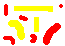
\includegraphics[width=0.6\linewidth]{images/strange7}}
    \caption[short]{}
\end{subfigure}%
\begin{subfigure}{.38\textwidth}
    \centering
    \fbox{
\includegraphics[width=0.8\linewidth]{images/rm/2}}
    \caption[short]{}
\end{subfigure}%
\begin{subfigure}{.38\textwidth}
    \centering
    \fbox{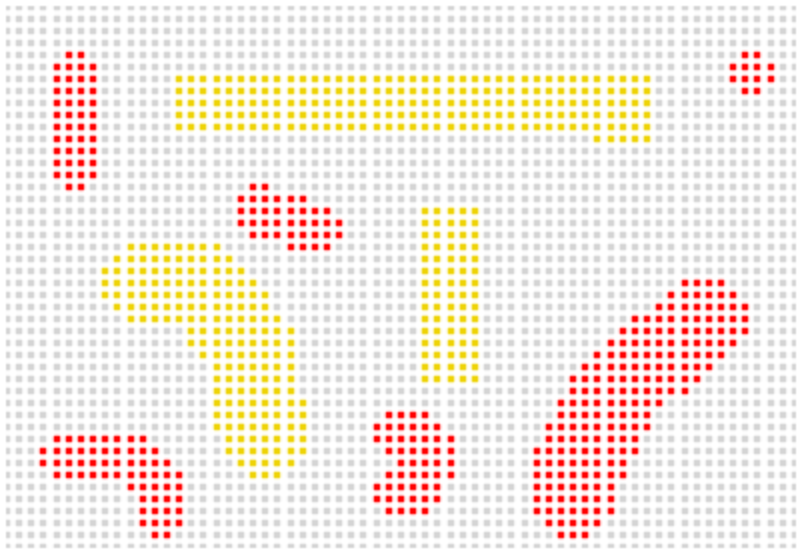
\includegraphics[width=0.8\linewidth]{images/rm/1}}
    \caption[short]{}
\end{subfigure}
\caption{Obrazek (a) przedstawia obrazek wejściowy w rzeczywistym rozmiarze. Obrazki (b) oraz (c) przedstawiają
powstały graf. Obrazek (b) przedstawia sposób podejścia do obszarów wyłączonych z obliczeń, gdzie nie tworzone są
odwzorowujące je wierzchołki, obrazek (c) pokazuje podejście gdzie w ich miejsce tworzone są wierzchołki z wagą $0$.
Dla czytelności wierzchołki zwykłe zostały oznaczone kolorem szarym. }
\label{im:input2}
\end{figure}

\begin{figure}[h]
\centering
\begin{subfigure}{.5\textwidth}
    \centering
    \fbox{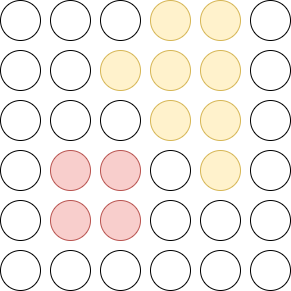
\includegraphics[width=0.6\linewidth]{images/in/1}}
    \caption[short]{}
\end{subfigure}
\begin{subfigure}{.5\textwidth}
    \centering
    \fbox{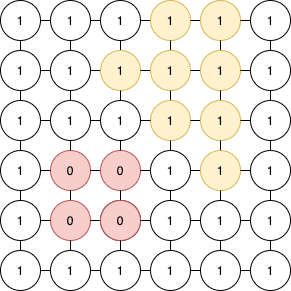
\includegraphics[width=0.6\linewidth]{images/in/2}}
    \caption[short]{}
\end{subfigure}%
\begin{subfigure}{.5\textwidth}
    \centering
    \fbox{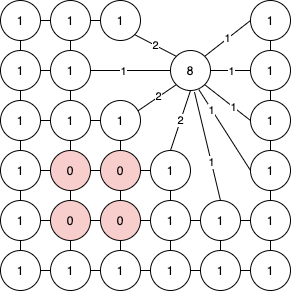
\includegraphics[width=0.6\linewidth]{images/in/3}}
    \caption[short]{}
\end{subfigure}
\begin{subfigure}{.5\textwidth}
    \centering
    \fbox{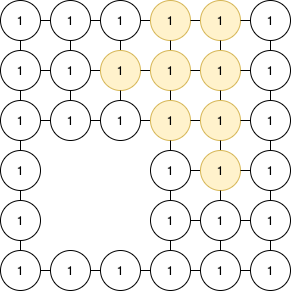
\includegraphics[width=0.6\linewidth]{images/in/4}}
    \caption[short]{}
\end{subfigure}%
\begin{subfigure}{.5\textwidth}
    \centering
    \fbox{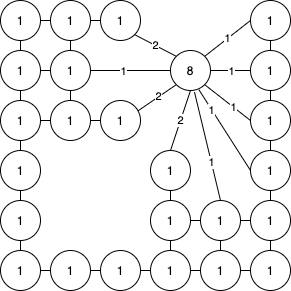
\includegraphics[width=0.6\linewidth]{images/in/5}}
    \caption[short]{}
\end{subfigure}
\caption{Obrazek (a) to wejściowa siatka.
Obszary niepodzielne są żółte, natomiast wyłączona z obliczeń czerwone.
Obrazek (b) oraz (d) pokazują siatkę tuż po konwersji na graf wedle dwóch sposobów.
Sposób (b) nadaje wierzchołkom na obszarach wyłączonych z obliczeń wagę $0$, natomiast sposób (d) usuwa wierzchołki obszarów
wyłączonych z obliczeń.
Na wierzchołkach zaznaczona jest waga.
Można zaobserwować wagę $1$ dla wierzchołków zwykłych i tych budujących obszary niepodzielne.
Na tym etapie wszystkie krawędzie mają wagę $1$. Obrazek (c) oraz (e) przedstawiają ten sam graf po redukcji obszarów
niepodzielnych, odpowiednio z kroku (b) oraz (d).
Wierzchołek, do którego został zredukowany obszar niepodzielny otrzymuje powiększoną wagę, równą sumie wag wierzchołków, które
redukuje. Niektóre krawędzie, które zastąpiły dwie krawędzie, zyskują sumę wag tych krawędzi równą $2$.}
\label{im:indivisible}
\end{figure}

\FloatBarrier



\newpage
\subsubsection{Zmniejszanie i partycjonowanie grafu za pomocą algorytmu LAM}

Aby stworzyć mniejszy odpowiednik wejściowego grafu stosowany jest algorytm tworzący skojarzenia (ang. matching).
Skojarzenie to podzbiór krawędzi grafu (ozn. $M$) o tej własności, że każdy wierzchołek jest końcem co najwyżej jednej krawędzi z $M$.
Pary wierzchołków połączone bezpośrednio krawędzią należącą do $M$ są skojarzone przez $M$ \cite{wiki:skojarzenie}.
\begin{figure}[h]
    \centering
    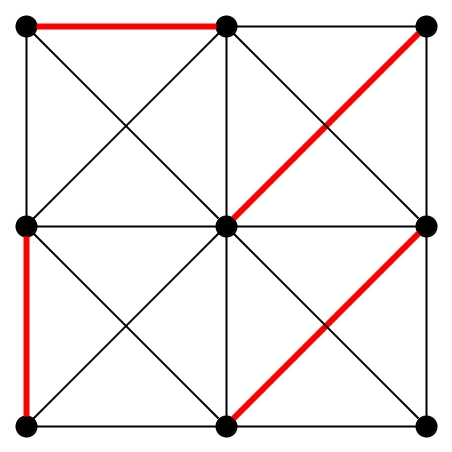
\includegraphics[width=0.24\linewidth]{images/Maximum_matching}
    \caption{Skojarzenie największe, którego liczba krawędzi wynosi 4.
    Źródło: \cite{wiki:skojarzenie}.}
    \label{im:max_skojarzenie}
\end{figure}

W celu zmniejszenia grafu stosowana jest heurystyka, która bazuje na metodzie \cite{weighted_maching}.
Algorytm ten oblicza $2$-approximation dla problemu maximum weighted matching w czasie liniowym.
Startuje on od arbitralnej krawędzi i sprawdza sąsiednie krawędzie.
Tak długo, jak jest w stanie znaleźć sąsiednią
krawędź z wyższą wagą, wywołuje się na niej i powtarza tę procedurę, aż znajdzie krawędź z lokalnie najwyższą wagą.
Ta krawędź łączy dwa wierzchołki, które zostaną skojarzone.
Skonstruowany w ten sposób algorytm dąży do budowania możliwie ''zwartych'' obszarów,
co oznacza to, że granice między obszarami są możliwie krótkie.
Krawędzie z wysokimi wagami łączą wierzchołki,
reprezentujące zbiory wierzchołków, które w początkowym grafie miały między sobą długą granicę.
Działanie algorytmu pokazany jest na rysunku \ref{im:lam_steps}.

\begin{figure}[h]
    \centering
    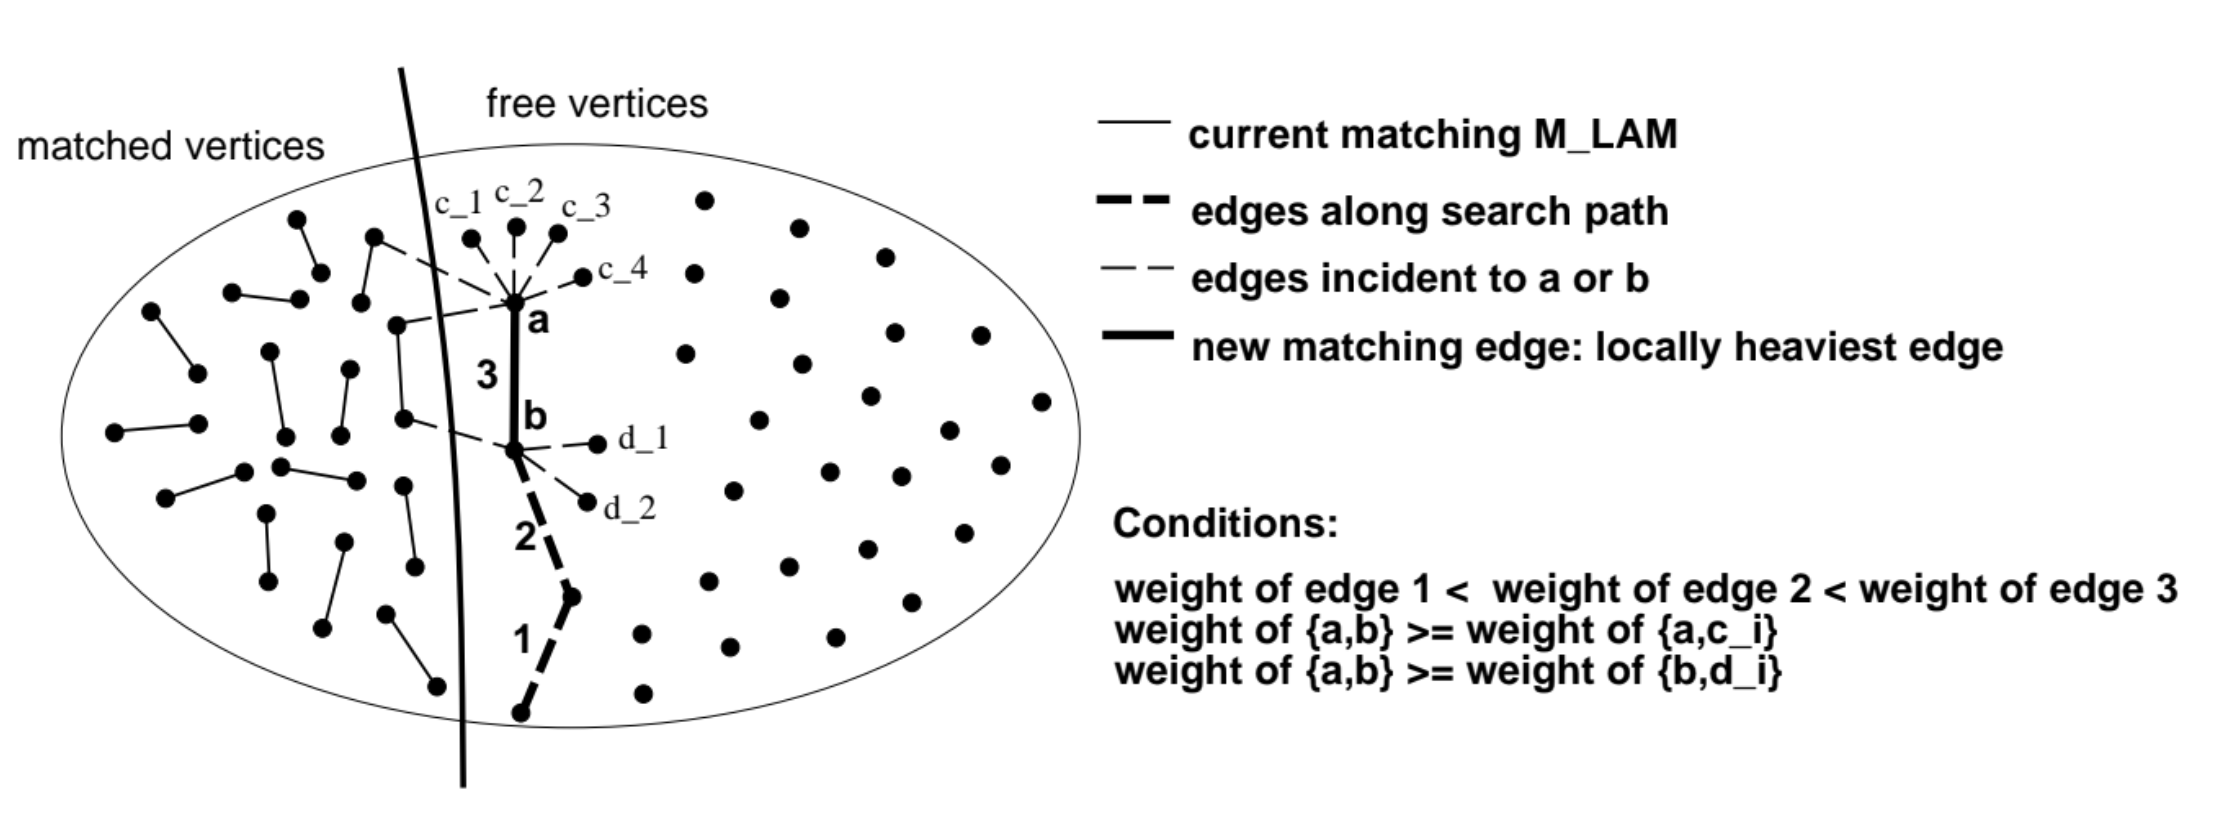
\includegraphics[width=0.9\linewidth]{images/lam}
    \caption{Fragment przebiegu algorytmu LAM. Startując od wybranej arbitralnie krawędzi numer $1$, ścieżka buduje się
    przez krawędzie z lokalnie wyższymi wagami - krawędź numer $2$ oraz $3$ -
    aż do znalezienia krawędzi \(\{a, b\}\) z lokalnie największą wagą. (Pokazywane są tylko krawędzie z aktualnego
    wywołania algorytmu LAM, krawędzi znajdujące się na ścieżce oraz krawędzie sąsiadujące do \(\{a, b\}\).
    Źródło: \cite{weighted_maching}.}
    \label{im:lam}
\end{figure}

\newpage
\begin{pseudocode}
@\underline{PROCEDURE shrink graph $(G)$}@
  t = 0 /* number of episodes */
  WHILE $|V_{G}|$ $\neq$ number of partitions we want to achieve
    matched_vertices = run LAM-Algorithm on $G$
    shrink $G$ based on the matched_vertices
    t = t + 1
  ENDWHILE


@\underline{LAM-Algorithm}@
  $M_{LAM} := \emptyset$; /* empty matching at the start */
  $U := E$; /* all edges are unchecked at the start */
  WHILE $(U \neq \emptyset)$
    take arbitrary edge $\{a,b\} \in U$;
    try match $(\{a,b\})$;
  ENDWHILE


@\underline{PROCEDURE try match $(\{a,b\})$}@
  $C_{\{a,b\}}(a) := \emptyset;$ $ C_{\{a,b\}}(b) := \emptyset;$ /* empty local sets of checked edges at the start */
  WHILE $(a$ is free AND $b$ is free AND $(\exists \{a,c\} \in U$ OR $\exists \{b,d\} \in U))$
    IF $(a$ is free AND $\exists \{a,c\} \in U)$
      move $\{a,c\}$ from $U$ to $C_{\{a,b\}}(a)$; /* move from U to C */
      IF $(w(\{a,c\}) > w(\{a,b\}))$
        try match $(\{a,c\})$; /* call heavier edge */
      ENDIF
    ENDIF
    IF $(b$ is free AND $\exists \{b,d\} \in U)$
      move $\{b,d\}$ from $U$ to $C_{\{a,b\}}(b)$; /* move from U to C */
      IF $(w(\{b,d\}) > w(\{a,b\}))$
        try match $(\{b,d\})$; /* call heavier edge */
      ENDIF
    ENDIF
  ENDWHILE
  IF $(a$ is free AND $b$ is free AND $\{a,b\}$ can be matched$)$
    add $\{a,b\}$ to $M_{LAM}$  /* new matching edge $\{a,b\}$ */
  ELSE IF $(a$ is matched AND $b$ is free$)$
    move edges $\{ \{b,d\} \in C_{\{a,b\}}(b)$ $|$ d is free$\}$ back to $U$;
  ELSE IF $(b$ is matched AND $a$ is free$)$
    move edges $\{ \{a,c\} \in C_{\{a,b\}}(a)$ $|$ c is free$\}$ back to $U$;
  ENDIF
\end{pseudocode}
\vspace{-8mm}
\captionof{listing}{Kod przedstawiający ulepszony algorytm LAM.
Wprowadzone przeze mnie zmiany dotyczyły warunku skojarzenia wierzchołków oraz końcowych
instrukcji warunkowych, które mogły zostać uproszczone z racji na brak potrzeby tworzenia zbioru krawędzi do usunięcia - $R$.
Niezmodyfikowany kod algorytmu można znaleźć w artykule \cite{weighted_maching}.}
\label{code:lam}
\newpage
Algorytm \ref{code:lam} (opisany w \cite{weighted_maching}) przedstawia procedury służące do zmniejszania grafu.
Końcowe efekty jego działania można obserwować na rysunku \ref{im:lam2} oraz \ref{im:lam_indivisible}.
Został ulepszony o bardziej rozbudowany warunek łączenia wierzchołków oraz uproszczony o usunięcie zbioru $R$, odpowiedzialny
za przechowywanie krawędzi do usunięcia.
Startuje z pustym zbiorem skojarzeń $M_{LAM}$.
Zbiór $U$ przechowuje nieodwiedzone krawędzie ($U = E$ na starcie).
Główną częścią algorytmu jest pętla WHILE (linia numer $13$), która wywołuje
procedurę 'try match' z arbitralnie wybraną, nieodwiedzoną krawędzią $\{a,b\}$.
Ta krawędź nie jest dodawana do
zbioru skojarzeń, dopóki wszystkie sąsiednie krawędzie prowadzące do wolnych wierzchołków (ang. free vertices) nie są sprawdzone
w zakresie poszukiwania nowej krawędzi z wyższą wagą - następuje to w pętli WHILE w linii numer $21$.
Każde wywołanie procedury 'try match $(\{a,b\})$' przechowuje swoje własne zbiory lokalnie odwiedzonych krawędzi
$C_{\{a,b\}}(a)$ oraz $C_{\{a,b\}}(b)$, w zależności od tego, czy nieodwiedzone krawędzie są sąsiadujące z wierzchołkiem
$a$ czy z $b$.
Jeśli wierzchołki $a$ i $b$ są wolne oraz co najmniej jeden z nich jest wierzchołkiem należącym do jednej z
nieodwiedzonych krawędzi, nieodwiedzona krawędź jest sprawdzana dalszymi instrukcjami.
Jeśli ma wyższą wagę od krawędzi $\{a,b\}$, 'try match' wywołuje się na niej rekursywnie.
Rekursywne wywołania są powtarzane aż do znalezienia krawędzi z lokalnie najwyższą wagą.
Następnie krawędź dodawana jest do $M_{LAM}$, a algorytm kończy aktualne wywołanie 'try match' i kontynuuje
pętlę WHILE sprawdzając kolejne sąsiadujące krawędzie.
Pętla WHILE kończy się wtedy, gdy $a$ oraz/lub $b$ zostaną skojarzone w rekursywnym wywołaniu, lub jeśli nie mają więcej
sąsiednich, nieodwiedzonych krawędzi. Następnie w końcowej części składającej się z instrukcji warunkowych
następuje sprawdzenie czy $a$ oraz $b$
są wolne. Jeśli tak, to $\{a,b\}$ jest dodawane do $M_{LAM}$.
W tej części, w oryginalnym algorytmie uzupełniany jest zbiór
wierzchołków do usunięcia \cite{weighted_maching} - $R$.
Ponadto jeśli $a$ lub $b$ są wolne, to wszystkie krawędzie, które zostały
odwiedzone w aktualnym wywołaniu, zawierające w sobie wierzchołek $a$ lub $b$, zostają oznaczone jako nieodwiedzone -
są przenoszone do zbioru $U$.

\begin{figure}[h]
\centering
\begin{subfigure}{.5\textwidth}
    \centering
    \fbox{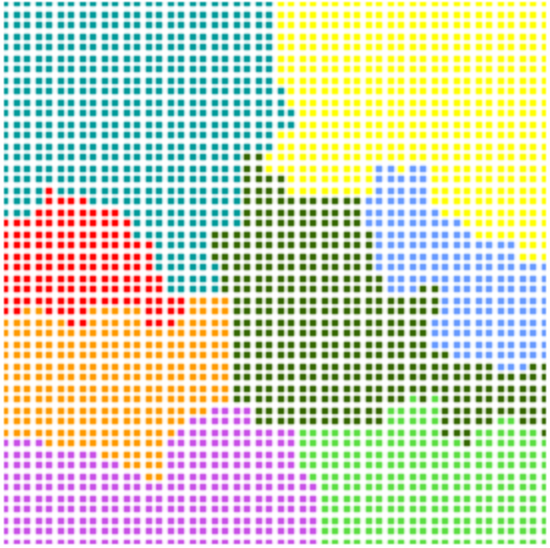
\includegraphics[width=0.6\linewidth]{images/lam-partitioning}}
    \caption[short]{partycjonowanie 1}
\end{subfigure}%
\begin{subfigure}{.5\textwidth}
    \centering
    \fbox{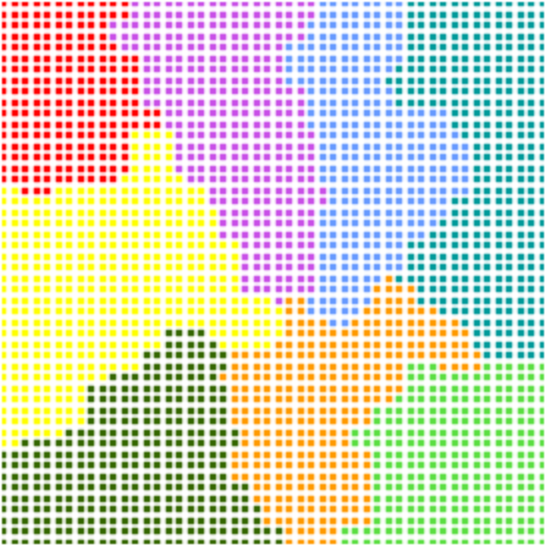
\includegraphics[width=0.6\linewidth]{images/lam-partitioning2}}
    \caption[short]{partycjonowanie 2}
\end{subfigure}
\caption{Dwa losowo wybrane partycjonowania siatki $50$x$50$ na $8$ obszarów za pomocą samego algorytmu LAM - bez fazy ulepszania podziału.
    Granice podziałów nie są optymalne, pola obszarów nie są równe, lecz bliskie bycia równym pod względem wielkości pól partycji, co jest
    oczekiwaną i dobrą bazą do dalszych operacji. Algorytm ma charakter losowy, co znaczy, że każde wywołanie
    będzie dawać inny rezultat. Zawsze jednak zachowane będzie dążenie do równych i zwartych obszarów.}
\label{im:lam2}
\end{figure}

Pętla WHILE w $21$ linii sprawdza krawędzie sąsiadujące z wierzchołkiem $a$ oraz $b$ tylko jeśli obydwa wierzchołki są wolne.
Ta cecha jest używana przez autorów artykułu do udowodnienia liniowej złożoności algorytmu.

Nieodwiedzone krawędzie zawarte w $U$ mają taką właściwość, że obydwa należące do nich wierzchołki są wolne.
Nowe krawędzie są przenoszone ponownie do $U$ w końcowej części z instrukcjami warunkowymi, ale tylko jeśli obydwa ich
wierzchołki są wolne.
Tak skonstruowany algorytm jest uruchamiany wielokrotnie przez procedurę 'shrink graph', aż do momentu, gdy liczba
wierzchołków w grafie osiągnie liczbę partycji, na które chcemy podzielić wejściową siatkę.
Po każdym wywołaniu algorytmu LAM uruchamiana jest procedura, która zamienia skojarzone pary wierzchołków na pojedyncze
wierzchołki wraz ze zmianą wagi.
Wyjątkiem jest ostatnie wywołanie, kiedy liczba wierzchołków w grafie osiąga wartość docelową.
Wtedy łączonych jest
pierwszych $n$ par wierzchołków, tak by otrzymać wymaganą liczbę wierzchołków.
Waga wierzchołka powstałego ze skojarzenia jest sumą wag wierzchołków kojarzonych.
Jeśli na skutek skojarzenia powstaje krawędź,
która zastępuje kilka krawędzi to jej waga jest sumą wag tych krawędzi.
Następnie do wierzchołków przyporządkowywane są numery partycji.
Zwykle jedno wywołanie algorytmu LAM
tworzy liczbę skojarzeń niewiele mniejszą niż połowa liczby wierzchołków w grafie.
W ten sposób graf, szczególnie w początkowych wywołaniach, zmniejszany jest o około połowę po każdym wywołaniu algorytmu LAM.
\vspace{mm}
\begin{figure}[h]
\centering
\begin{subfigure}{.5\textwidth}
    \centering
    \fbox{
\includegraphics[width=0.8\textwidth]{images/lam-obszary-niepodzielne/grid}}
    \caption[short]{siatka do partycjonowania}
\end{subfigure}%
\begin{subfigure}{.5\textwidth}
    \centering
    \fbox{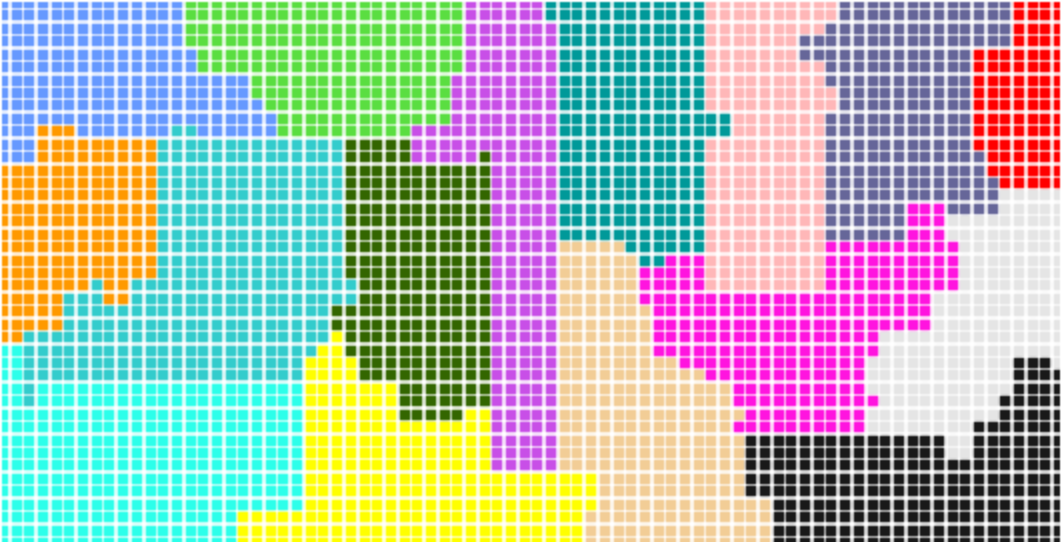
\includegraphics[width=0.8\textwidth]{images/lam-obszary-niepodzielne/4}}
    \caption[short]{partycjonowanie}
\end{subfigure}
\caption{Obrazek (b) przedstawia partycjonowanie siatki (a) samym algorytmem LAM. Widoczne jest uwzględnianie obszarów
niepodzielnych, które na siatce (a) zaznaczone są jako obszary żółte.}
\label{im:lam_indivisible}
\end{figure}

\newpage
\newcommand\imgs{0.43}
\begin{figure}[h]
\begin{subfigure}{.5\textwidth}
    \centering
    \fbox{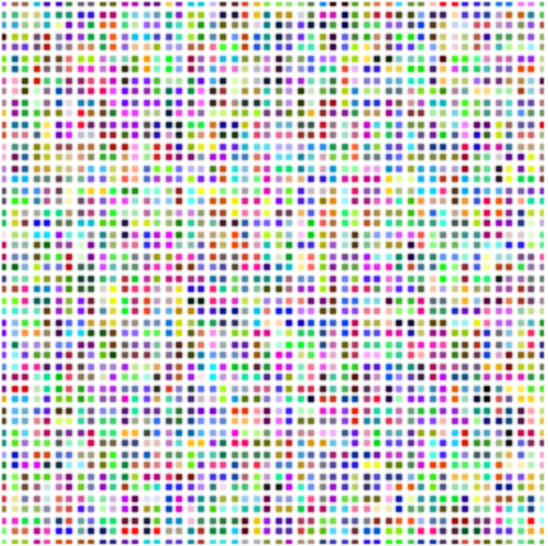
\includegraphics[width=\imgs\textwidth]{images/part-steps/lam1}}
    \caption[short]{krok 1}
\end{subfigure}
\begin{subfigure}{.5\textwidth}
    \centering
    \fbox{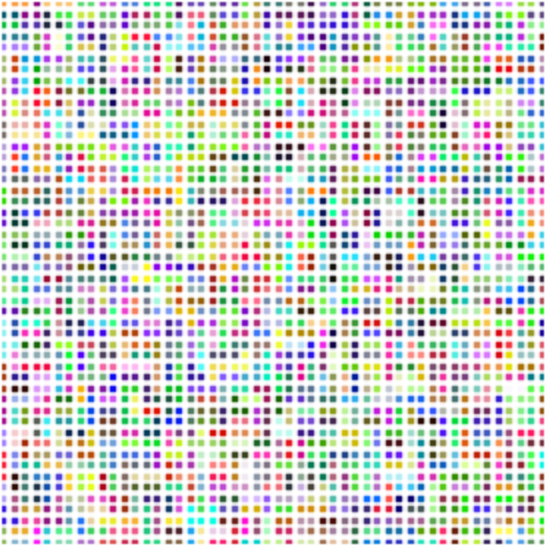
\includegraphics[width=\imgs\textwidth]{images/part-steps/lam2}}
    \caption[short]{krok 2}
\end{subfigure}%

\begin{subfigure}{.5\textwidth}
    \centering
    \fbox{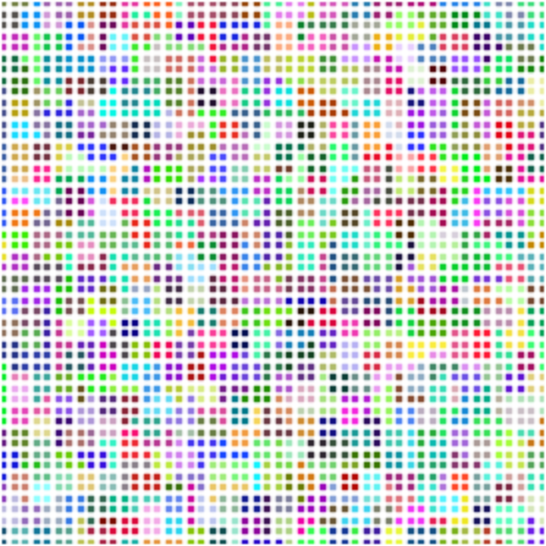
\includegraphics[width=\imgs\textwidth]{images/part-steps/lam3}}
    \caption[short]{krok 3}
\end{subfigure}
\begin{subfigure}{.5\textwidth}
    \centering
    \fbox{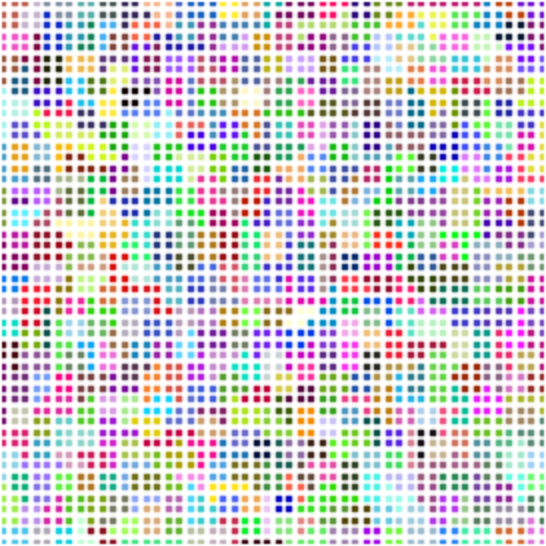
\includegraphics[width=\imgs\textwidth]{images/part-steps/lam4}}
    \caption[short]{krok 4}
\end{subfigure}%

\begin{subfigure}{.5\textwidth}
    \centering
    \fbox{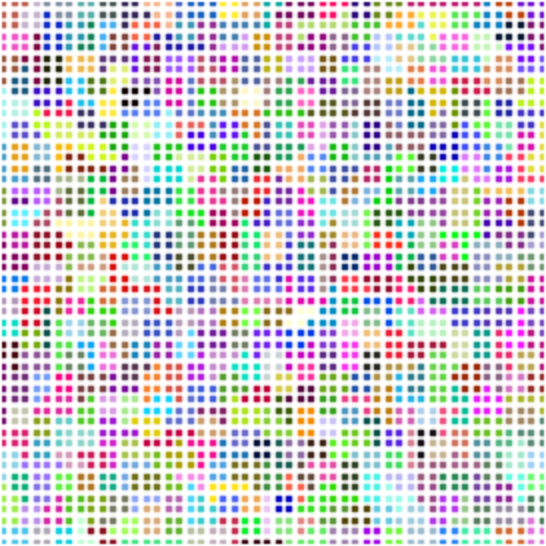
\includegraphics[width=\imgs\textwidth]{images/part-steps/lam5}}
    \caption[short]{krok 5}
\end{subfigure}
\begin{subfigure}{.5\textwidth}
    \centering
    \fbox{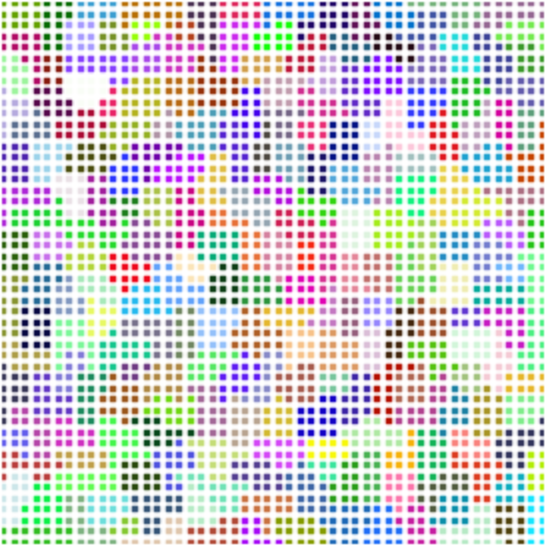
\includegraphics[width=\imgs\textwidth]{images/part-steps/lam6}}
    \caption[short]{krok 6}
\end{subfigure}%

\begin{subfigure}{.5\textwidth}
    \centering
    \fbox{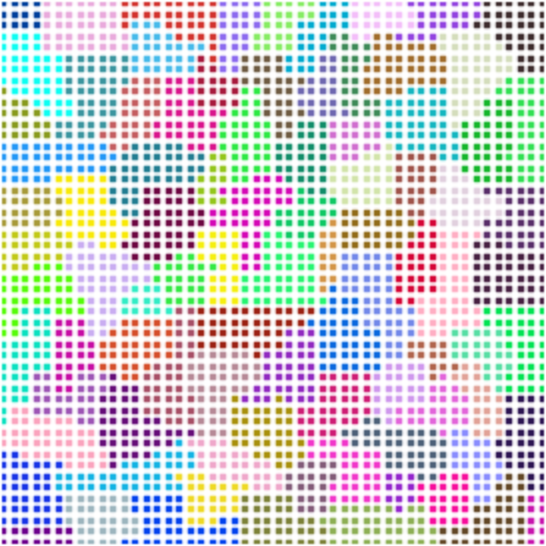
\includegraphics[width=\imgs\textwidth]{images/part-steps/lam7}}
    \caption[short]{krok 7}
\end{subfigure}
\begin{subfigure}{.5\textwidth}
    \centering
    \fbox{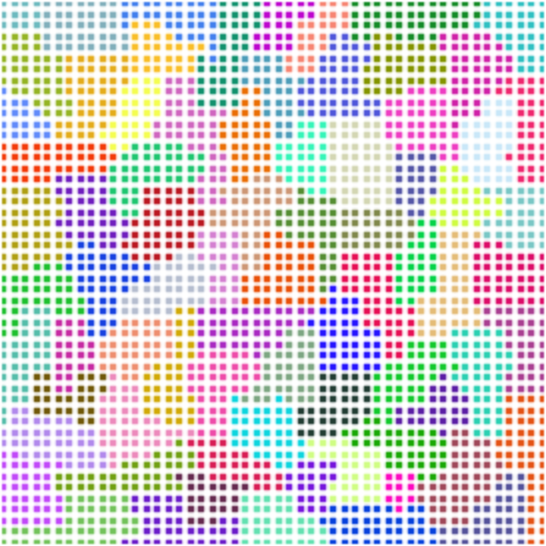
\includegraphics[width=\imgs\textwidth]{images/part-steps/lam8}}
    \caption[short]{krok 8}
\end{subfigure}%

\begin{subfigure}{.5\textwidth}
    \centering
    \fbox{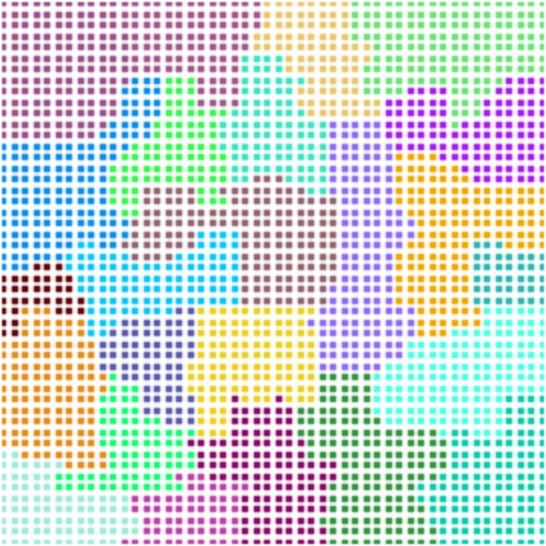
\includegraphics[width=\imgs\textwidth]{images/part-steps/lam9}}
    \caption[short]{krok 9}
\end{subfigure}
\begin{subfigure}{.5\textwidth}
    \centering
    \fbox{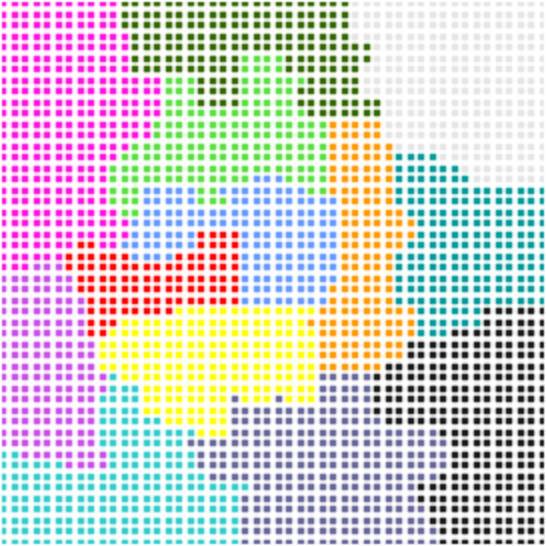
\includegraphics[width=\imgs\textwidth]{images/part-steps/lam10}}
    \caption[short]{krok 10}
\end{subfigure}
\caption{Obrazki przedstawiają wybrane, kolejne kroki algorytmu LAM aż do otrzymaniu podziału siatki $50$x$50$ na $13$ obszarów.
Przedstawione zostało co siódme wywołanie algorytmu oraz efekt końcowy. Widoczne jest równomierne łączenie obszarów.}
\label{im:lam_steps}
\end{figure}
\FloatBarrier
\newpage
\subsubsection{Szczegóły modyfikacji algorytmu LAM}
Algorytm ten bez dodatkowego warunku na skojarzenie wierzchołków (linia $35$) zwykle tworzyłby grafy typu gwiazda, co oznacza,
że powstawałaby część wierzchołków o bardzo wysokim stopniu.
To powodowałoby, że zmniejszony graf nie przypominałby początkowego grafu.
Warunek ten został dodany przez autorów artykułu \cite{weighted_maching} i mówi, że
skojarzenie wierzchołka $a$ z wierzchołkiem $b$ może zaistnieć tylko wtedy, jeśli ich sumaryczna
waga nie przekracza dwukrotności najmniejszej wagi wierzchołka w grafie,
zsumowanej z największą wagą wierzchołka w grafie.
\begin{equation}
w_{a} + w_{b} \leq w_{highest} + 2 \cdot w_{lowest}
\label{eq:condition1}
\end{equation}
Warunek \ref{eq:condition1} powoduje, że nawet jeśli rozpatrujemy skojarzenie wierzchołka o relatywnie wysokiej wadze, to ma on szansę
zostać skojarzony jedynie z wierzchołkiem o wadze niskiej, co prowadzi do równiejszych wag w grafie.
W dalszych etapach zmniejszania grafu trudniej spełnić
warunek na skojarzenie wierzchołków - pojawia się więcej różnorodności w zakresie wag wierzchołków grafu, a co za tym idzie,
spada liczba udanych skojarzeń przypadających na wywołanie.
Kiedy zbyt mało par jest kojarzonych podczas pojedynczego wywołania, warunek ten jest osłabiany poprzez
zwiększenie dopuszczalnej sumarycznej wagi wierzchołka $a$ oraz $b$.

Warunek stworzony przez autorów artykułu \cite{weighted_maching} okazał się nie działać w kontekście obszarów
niepodzielnych.
W tym celu stworzony został nowy, zmodyfikowany warunek \ref{eq:condition3}, bazujący na warunku \ref{eq:condition1}
rozszerzonym o $discount$ (wzór \ref{eq:condition2}).
\begin{equation}
discount = \frac{t}{T \cdot \frac{w_{highest}}{w_{lowest} + 1} \cdot \log(number\_of\_partitions) + 1}
\label{eq:condition2}
\end{equation}
Jeśli $discount > 1$ wtedy ma przypisywaną wartość $1$.
$T$ to przewidywana liczba wywołań algorytmu LAM.
Obliczana jest jako liczba dzieleń liczby wierzchołków grafu przez liczbę dwa, potrzebna do uzyskania liczby wierzchołków mniejszej
lub równej docelowej liczbie partycji.
$t$ to licznik wywołań algorytmu LAM (linia $2$).
Z użyciem $discountu$ powstał zmodyfikowany przeze mnie warunek na skojarzenie wierzchołków $a$ i $b$:
\begin{equation}
w_{a} + w_{b} \leq discount \cdot (w_{highest} + 2 \cdot w_{lowest})
\label{eq:condition3}
\end{equation}
Niedziałanie poprzedniego warunku jest spowodowane faktem,
iż w początkowej fazie algorytmu, tuż po zamianie wejściowej siatki na graf,
wszystkie obszary niepodzielne zamieniane są na pojedyncze wierzchołki.
Waga dla wierzchołków reprezentujących obszary niepodzielne jest równa sumie wag wierzchołków, które do nich należą.
Oryginalny algorytm LAM został zaprojektowany z założeniem równomiernego budowaniu skojarzeń ze względu na wagi wierzchołków w grafie
od samego początku.
W warunku na skojarzenie wierzchołków bierze pod uwagę wierzchołek z aktualnie największą wagą
oraz aktualnie najmniejszą wagą w grafie.
Warunek ten funkcjonuje poprawnie, jeśli graf jest zmniejszany równomiernie od samego początku, kiedy wagi wszystkich
wierzchołków w grafie mają taką samą lub niemal taką samą wartość.
W momencie, w którym na samym początku pojawiają się wierzchołki o dużych wagach (z powodu zamiany wierzchołków
należących do obszarów niepodzielnych na pojedyncze wierzchołki o wyższych wagach) warunek \ref{eq:condition1} zaczyna
działać niepoprawnie.
W szczególnym przypadku, jeśli taki obszar zajmuje więcej niż połowę całej siatki
(rysunek \ref{im:discount}) niemal każde skojarzenie dwóch wierzchołków, z których żaden nie jest
reprezentującym obszar niepodzielny, będzie dozwolone.
Każdy z takich wierzchołków ma bowiem wagę mniejszą niż suma podwojonej najmniejszej i największej
wagi wierzchołka w grafie.
Warunek \ref{eq:condition1} jest więc niemal zawsze spełniony.
W tego typu przypadkach realny podział odbywa się tak naprawdę poza obszarem niepodzielnym, ponieważ wiemy, że będzie on
na końcu jedną partycją, a jako że jest największym wierzchołkiem w grafie - nie będzie mógł tworzyć
wielu skojarzeń.
Prowadzi to do kojarzenia obszarów bez zachowania równomiernych pól jak na rysunku \ref{im:discount}(b).
W efekcie w skład wielu partycji wchodzi tylko jeden wierzchołek.

Zaproponowana przeze mnie modyfikacja (wzór \ref{eq:condition2}), polegająca na dodaniu $discountu$,
wzmacnia warunek
i powoduje bardziej równomierne (ze względu na wagi) łączenie się wierzchołków.
$discount$ zależny jest od liczby iteracji - osłabia się w czasie.
Im późniejsza iteracja tym bliższy jest wartości $1$,
a więc zmierza do oryginalnego warunku \ref{eq:condition1}.
Ważne jest jednak, że w kluczowych, początkowych wywołaniach algorytmu LAM pozwala na równomierne skojarzenia.
Efekt działania warunku widoczny jest na rysunku \ref{im:discount}.
\vspace{8mm}
\begin{figure}[h]
\centering
\begin{subfigure}{.5\textwidth}
    \centering
    \fbox{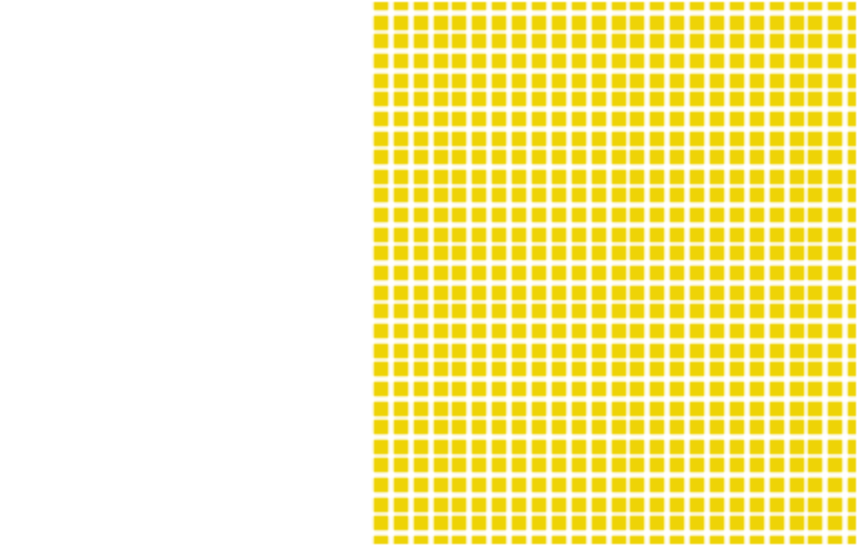
\includegraphics[width=0.7\textwidth]{images/discount1}}
    \caption[short]{siatka do partycjonowania}
\end{subfigure}%
\begin{subfigure}{.5\textwidth}
    \centering
    \fbox{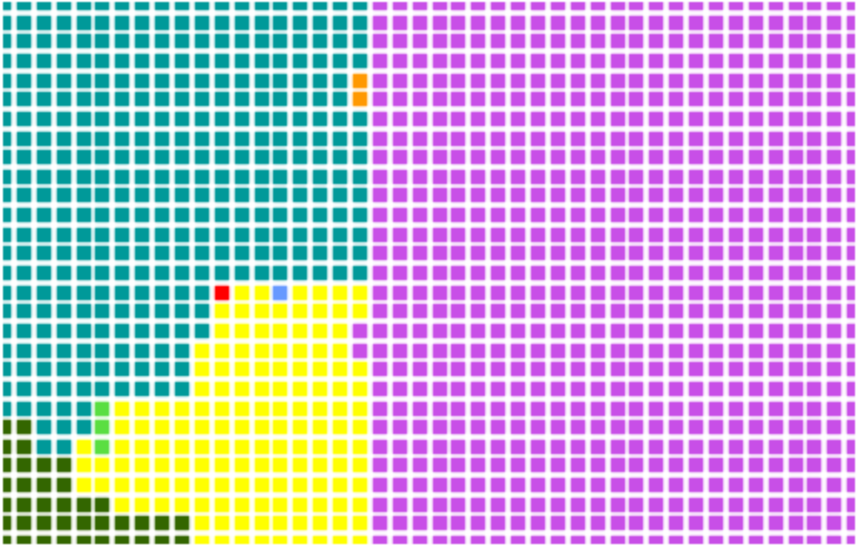
\includegraphics[width=0.7\textwidth]{images/discount2}}
    \caption[short]{partycjonowanie 1 bez użycia discountu}
\end{subfigure}
\begin{subfigure}{.5\textwidth}
    \centering
    \fbox{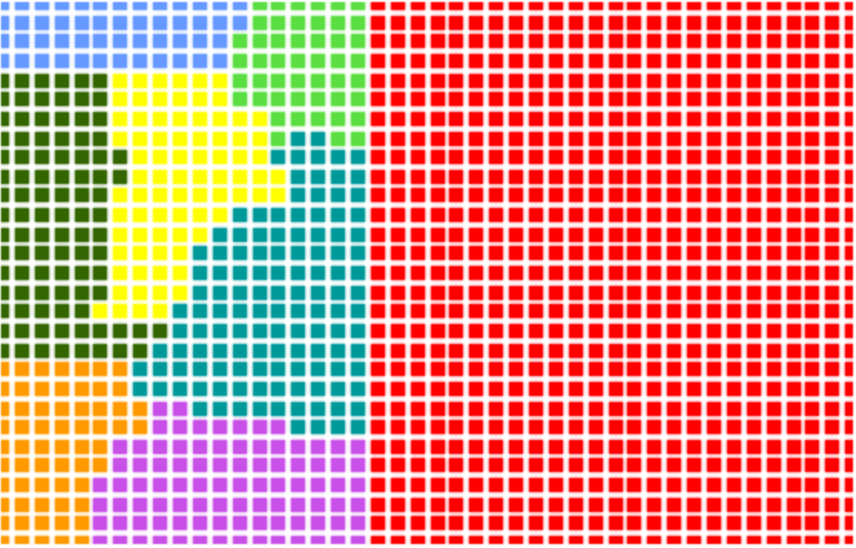
\includegraphics[width=0.7\textwidth]{images/discount3}}
    \caption[short]{partycjonowanie 2 z użyciem discountu}
\end{subfigure}%
\begin{subfigure}{.5\textwidth}
    \centering
    \fbox{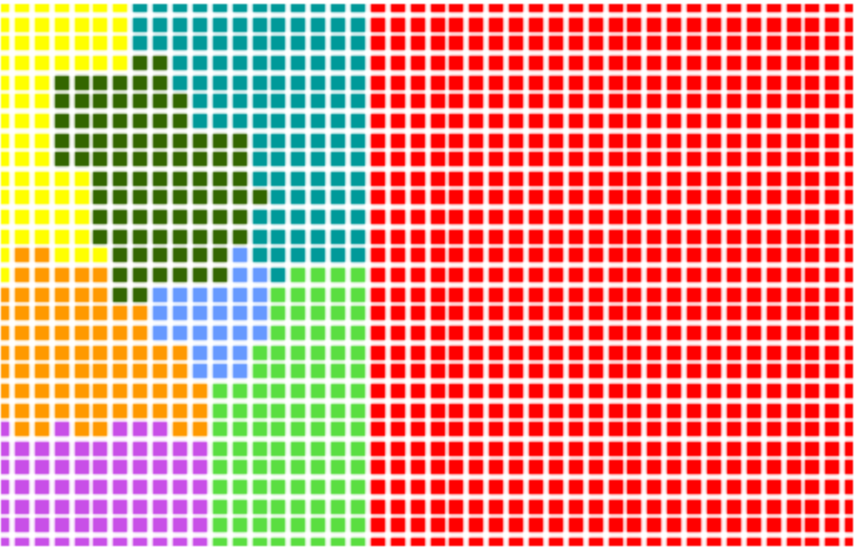
\includegraphics[width=0.7\textwidth]{images/discount4}}
    \caption[short]{partycjonowanie 3 z użyciem discountu}
\end{subfigure}
\caption{Obrazek (a) przedstawia siatkę wejściową, której więcej niż połowę zajmuje oznaczony kolorem żółtym obszar niepodzielny.
Obrazek (a), (b) oraz (c) przedstawia partycjonowanie siatki na 8 części wykonane algorytmem LAM bez fazy ulepszania podziału.
Obrazek (b) pokazuje partycjonowanie wykonane z użyciem warunku \ref{eq:condition1} na skojarzenie wierzchołków.
Obraz (c) oraz (d) prezentuję partycjonowanie wykonane z użyciem warunku \ref{eq:condition3}.}
\label{im:discount}
\end{figure}

\newpage
Negatywnym efektem stosowania $discountu$ jest większa liczba wywołań algorytmu LAM.
Czasami zmienna $t$ musi urosnąć
do konkretnej wartości, umożliwiającej dokonanie kolejnych, blokowanych obecnie skojarzeń, a żadne inne skojarzenia,
które spełniałyby warunek nie są w danej chwili możliwe.
Rysunek \ref{im:discount} pokazuje pozytywne działanie modyfikacji na jakość podziału wraz z porównaniem do poprzedniej
wersji warunku.

Skonstruowanie $discountu$ polegało na odpowiednim dobraniu jego wartości względem parametrów dzielonej siatki, tak by
nie działał zbyt agresywnie, nadmiernie przedłużając obliczenia, a jednocześnie był na tyle agresywny, aby pozwalał tylko na
kojarzenie wierzchołków prowadzące do możliwie równych podziałów.
Został skonstruowany na bazie podstawowego współczynnika $\frac{t}{T}$, który na podstawie wielu prób
dostosowałem dodatkowymi zmiennymi w poszukiwaniu wcześniej opisywanego balansu.
W momencie, gdy partycjonujemy obszar, w którym nie ma dużych obszarów niepodzielnych, nie musimy stosować
$discountu$.
W takim wypadku jedynym jego efektem będzie większa liczba wywołań algorytmu LAM.



\newpage
\subsubsection{Przywracanie grafu do początkowego rozmiaru wraz z ulepszeniem podziału}

Kolejną częścią algorytmu jest faza przywracania grafu do początkowej wielkości.
Tej fazie towarzyszy poprawianie podziału, które polega na zmniejszaniu długości granic oraz na
wyrównywaniu wielkości pól pomiędzy obszarami.
Ten etap nadaje podziałowi ostateczny kształt.
W tym celu zaimplementowana została zmodyfikowana heurystyka Helpful Sets (HS) \cite{10.1007/3-540-44842-X_6}.
Efekt jej działania widoczny jest na rysunku \ref{im:refinement}.
\vspace{2mm}
\begin{figure}[h]
\centering
\begin{subfigure}{.5\textwidth}
    \centering
    \fbox{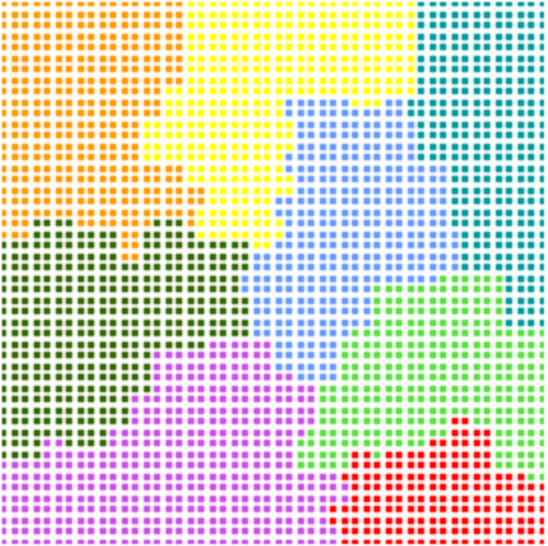
\includegraphics[width=0.4\textwidth]{images/refinement/1}}
    \caption[short]{po algorytmie LAM}
\end{subfigure}%
\begin{subfigure}{.5\textwidth}
    \centering
    \fbox{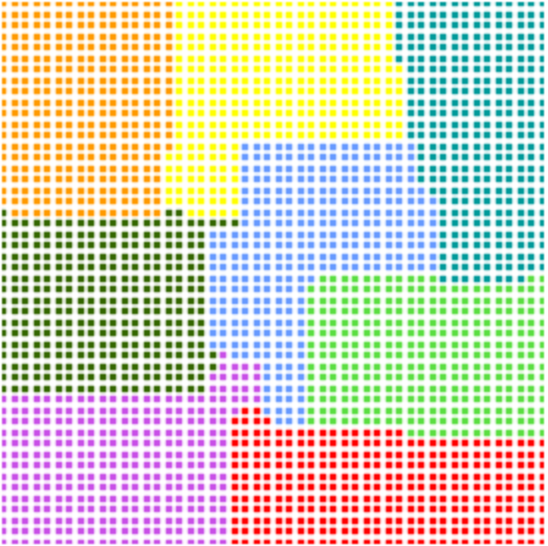
\includegraphics[width=0.4\textwidth]{images/refinement/2}}
    \caption[short]{po fazie ulepszania}
\end{subfigure}
\caption{Obrazek (a) przedstawia partycjonowanie siatki (a) samym algorytmem LAM.
Obrazek (b) przedstawia ulepszenie podziału z obrazka (a). Zmniejszona została długość granic oraz wyrównane zostały pola.}
\label{im:refinement}
\end{figure}


Etap pierwszy to heurystyka HS do poprawiania podziału. Jest oparata na wyszukiwaniu lokalnym -
próbuje poprawić aktualny podział poprzez wielokrotne wprowadzanie lokalnych zmian. Wierzchołki klasyfikowane są
pod kątem liczby krawędzi z wierzchołkami obszaru do którego należą (ang. internal edges) oraz z wierzchołkami
pozostałych obszarów (ang. external edges).
Wedle tej klasyfikacji wierzchołki przy granicach wymieniane są między obszarami.
Niech $A$ i $B$ będą partycjami na siatce.
Algorytm dzieli się na dwie fazy.
Pierwsza buduje zbiór wierzchołków $C$ na wierzchołkach partycji $A$, a następnie przenosi go z partycji $A$ do partycji $B$.
Wierzchołki są dobierane tak, aby zmniejszyć długość granicy między obszarami.
Druga faza to faza szukania zbioru balansującego $D$.
Jest budowany na zbiorze $B$.
Jego celem jest zwrócenie zbioru wierzchołków z partycji $B$ do partycji $A$ o tej samej wielkości jak zbiór $C$
z jednoczesnym możliwie utrzymanym ulepszeniem w długości granicy po wcześniejszej fazie.
Zbiór $C$ nazywamy \texttt{k-helpful set}, natomiast zbiór $D$ nazywamy \texttt{balancing set}.
Po etapie ulepszenia granicy następuje etap drugi mający na celu wyrównywanie pól.
Używając tej samej klasyfikacji wierzchołki przy granicach przenoszone są z obszarów mniejszych do większych.
Te dwa etapy powtarzane są co jakiś czas podczas przywracania grafu do początkowej wielkości.
Najpierw więc pracują na grafie o mniejszej liczbie wierzchołków gdzie każdy wierzchołek reprezentuje zbiór wierzchołków.
W ten sposób w formie pojedynczych wierzchołków o dużych wagach efektywnie przenoszone są duże obszary.
Im dalej w procesie przywracania grafu tym algorytm pracuje na większym grafie z wierzchołkami o mniejszych wagach.
Podział jest już ulepszony w poprzednich wywołaniach więc może skupić się na bardziej lokalnych poprawkach.
\newpage
\begin{pseudocode}
@\underline{PROCEDURE RestoreGraphWithPartitionsImprovements}@
  $number\_of\_restoration\_steps\_done$ $\leftarrow$ $0$
  $number\_of\_all\_reductions$ $\leftarrow$ $reductions$.$length$
  WHILE $number\_of\_all\_reductions$ $-$ $number\_of\_restoration\_steps\_done$ $>$ $0$
    $reduction$ $=$ $reductions$.$pop()$
    RestoreReduction$(reduction)$
    $number\_of\_restoration\_steps\_done$ $\leftarrow$ $number\_of\_restoration\_steps\_done$ $+$ $1$
    IF $number\_of\_restoration\_steps\_done$ $/$ $number\_of\_all\_reductions$ $>$ $0.9$ AND
       floor$(number\_of\_all\_reductions$ mod $($$number\_of\_all\_reductions$ $\cdot$ $0.03))$ $==$ $0$
      ImprovePartitioning
    ENDIF
  ENDWHILE
  ImprovePartitioning
  WHILE there are any indivisible areas:
    area $\leftarrow$ pop one of them
    RestoreReduction(area)
  ENDWHILE
\end{pseudocode}
\vspace{-8mm}
\captionof{listing}{Algorytm przedstawia główną procedure optymalizującą długość granic.}
\label{code:main_impr_procedure}
\vspace{4mm}
Na algorytmie \ref{code:main_impr_procedure}
przedstawiona jest główna procedura odpowiedzialna za przywrócenie grafu do
początkowej wielkości wraz z wprowadzaniem optymalizacji granic.
Autorzy artykułu \cite{1364754}, na podstawie którego stworzona została niniejsza praca, wyspecyfikowali, że
do optymalizacji granic używany jest algorytm HelpfulSets, który
wywoływany jest wielokrotnie na różnych etapach przywracania grafu.
Nie było natomiast informacji na temat tego, jak często ten algorytm jest wywoływany oraz w jakich stadiach przywracania grafu.
W związku z powyższym zaproponowałem wyżej wymienione rozwiązanie.
Dodatkową modyfikacją algorytmu przywracania grafu było również wzięcie pod uwagę obszarów niepodzielnych.
Pierwsza pętla WHILE (linia $4$) odpowiedzialna jest za przywrócenie zwykłych
redukcji, to znaczy tych, które zostały stworzone przez algorytm LAM oraz wprowadzenie ulepszeń.
Inne redukcje to te, które wykonywane są na obszarach niepodzielnych zaraz po
algorytmie, który zamienia obrazek przedstawiający siatkę na graf - te przywracane są na samym końcu po przeprowadzeniu
optymalizacji granic.

Procedura \texttt{ImprovePartitioning} za każdym razem aktualizuje informacje o sąsiadujących obszarach, ponieważ
te mogą ulec zmianie na skutek kolejnych wywołań algorytmu, a następnie iteruje po wszystkich parach sąsiadujących obszarów i wywołuje
dla nich procedurę \texttt{HelpfulSet}.
Pseudokod procedury \texttt{HelpfulSet} został przedstawiony na algorytmie \ref{code:helpful_sets}.
Jak wynika z kodu (linia $8$) proces optymalizacji długości granic oraz pól obszarów zaczyna się dopiero,
gdy graf przywrócony jest przynajmniej w $90\%$.
Tą wartością można manipulować dowolnie, jednak powinna być ona wysoka.
W momencie, kiedy pozwolimy algorytmowi optymalizować bardzo zredukowane grafy, to przesuwane na raz są bardzo duże pule wierzchołków.
Algorytm do optymalizacji granic stworzony został raczej, żeby wprowadzać małe lokalne zmiany, niż przesuwać duże obszary,
szybko więc w takiej sytuacji niszczy podział zamiast go poprawiać.
Efektem takiego niszczenia są obszary, które podzielone są na dwie części.
Zjawisko to przedstawione jest na rysunku \ref{im:noises} i będzie dokładnej opisany w dalszych częściach pracy.
W linii $9$ widzimy także, że optymalizacja przeprowadzana jest co pewną liczbę przywróconych redukcji.
Przywrócenie jednej redukcji bowiem, to zamiana jednego wierzchołka na dwa wierzchołki, które zastąpiła, a więc
jest to za mała zmiana, żeby ponownie włączać optymalizację na całym grafie.
Na podstawie doświadczenia mogę stwierdzić, że współczynniki winny być ustawione tak, aby wywoływać
algorytm optymalizacji granic $5$-$10$ razy podczas przywracania grafu.
Takie wartości gwarantują dobry wynik przy niezbyt długim czasie wykonania.
Więcej wywołań niekoniecznie da nam lepszy rezultat.
Ta funkcjonalność została zaimplementowana przez użyciu operacji wyliczania reszty z dzielenia.
W linii $13$ następuje ostatnie wywołanie algorytmu optymalizacji granic już na niemal całkowicie przywróconym grafie
(nie licząc obszarów niepodzielnych).
Ostatnim krokiem jest przywrócenie obszarów niepodzielnych, co dzieje się w drugiej pętli WHILE
w linii $14$.
\newpage
\subsubsection{Używanie Helpful Sets w celu zmniejszenia długości granic}
Heurystyka Helpful Sets startuje od początkowego podziału i za pomocą lokalnie wprowadzanych zmian zmniejsza długość granic.
Algorytm startuje od poszukiwania zbioru \texttt{k-helpful}, to jest podzbioru wierzchołków ze zbioru $V_1$ lub $V_2$,
który zmniejsza długość granicy o $k$, jeśli zostanie przeniesiony do drugiej partycji.
Jeśli taki zbiór zostaje znaleziony w jednej z dwóch
partycji, na przykład w $V_1$, to jest przenoszony do $V_2$.
Następnie algorytm zaczyna szukać w części $V_2$, która
jest aktualnie wystarczająco duża, aby zbalansować podział i zwiększyć długość granicy o maksymalnie $(k-1)$ krawędzi.
Jeśli taki \texttt{balancing set} zostaje znaleziony, to przenoszony jest do zbioru $V_1$ i proces zaczyna się od początku.
Działanie algorytmu dobrze widać na rysunku \ref{im:balancing} oraz \ref{im:h_steps}.
Zanim algorytm zostanie opisany dokładniej, potrzebne są definicje zbiorów helpful oraz balancing:

\begin{definition}
(diff-value wierzchołka)\newline
Dla wierzchołka $v \subset V$ wartość diff-value definiujemy jako $diff(v) = ext(v) - int(v)$.
\end{definition}

\begin{definition}
(Helpful Set)\newline
Niech $S \subset V_i, i \in \{1,2\}$ będzie podzbiorem wierzchołków partycji. Dla każdego $v \in S$ definiujemy
$int_s(v) = |\{w \in S; \{v,w\} \in E\}|$ - zbiór krawędzi wewnętrznych $S$.

\begin{equation}
H(S)=\sum_{v \in S}(ext(v) - int(v) + int_s(v))
\label{eq:helpful_set2}
\end{equation}
to \textbf{helpfulness} zbioru S. Zbiór S nazywany jest H(S)-\textbf{helpful}.
\end{definition}

Przeniesienie zbioru $S$ do drugiej partycji zmniejsza długość granicy o $H(S)$.
Przykłady zbiorów $2$-helpful pokazane są na rysunku \ref{im:helpfulsets:example}.

Autorzy artykułu \cite{article} zamienne używają pojęć diff-value oraz helpfulness.
W niniejszej pracy używana jest nazwa helpfulness zarówno dla wierzchołków, jak i dla zbiorów.

\begin{figure}[h]
\centering
\begin{subfigure}{.3\textwidth}
    \centering
    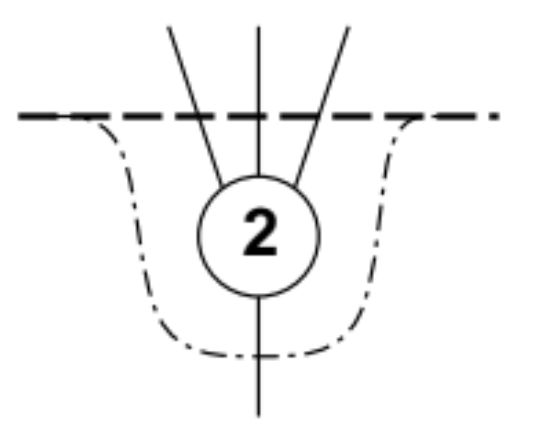
\includegraphics[width=0.55\textwidth]{images/helpfulsets/1}
    \caption[short]{}
\end{subfigure}
\begin{subfigure}{.69\textwidth}
    \centering
    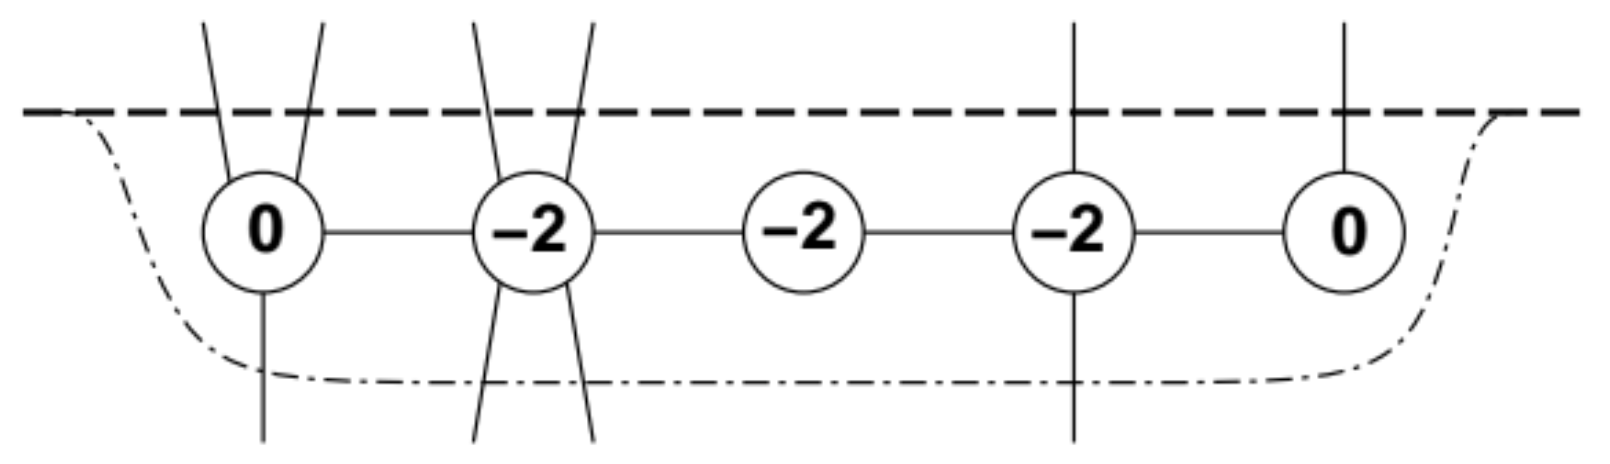
\includegraphics[width=0.68\textwidth]{images/helpfulsets/2}
    \caption[short]{}
\end{subfigure}%

\begin{subfigure}{.4\textwidth}
    \centering
    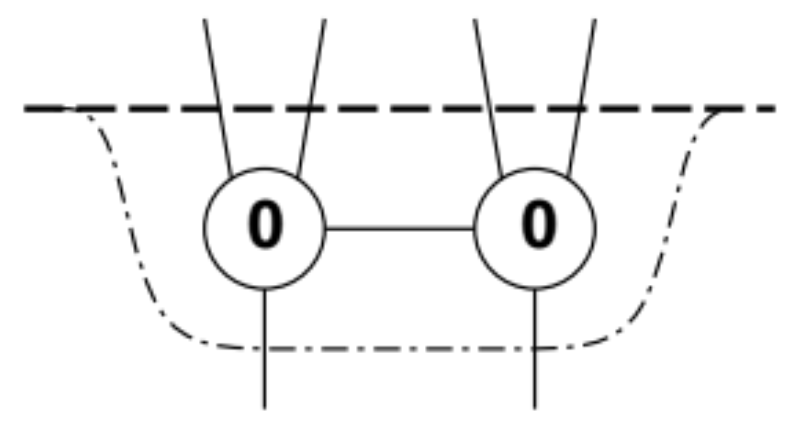
\includegraphics[width=0.63\textwidth]{images/helpfulsets/3}
    \caption[short]{}
\end{subfigure}
\begin{subfigure}{.59\textwidth}
    \centering
    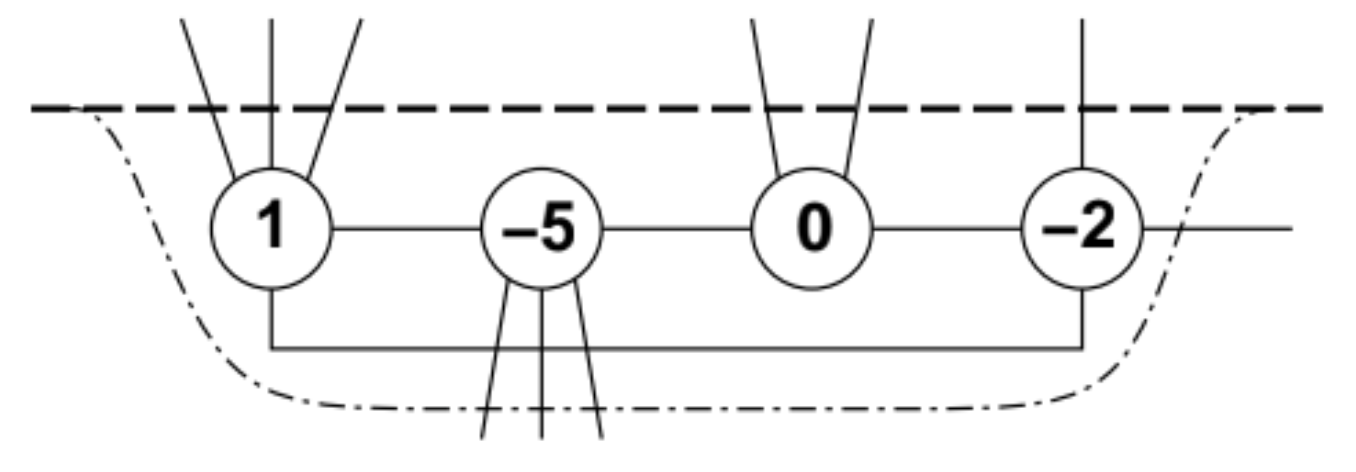
\includegraphics[width=0.68\textwidth]{images/helpfulsets/4}
    \caption[short]{}
\end{subfigure}
\caption{Zbiory 2-helpful. Na górze każdego z 4 przykładów jest zbiór zewnętrzny (ang. external set). Wyliczanie wartości
helpfulness na podstawie wzoru \ref{eq:helpful_set2}: (a): $3-1+0=2$, (b): $6-8+4=2$, (c): $4-3+1=2$ oraz (d): $6-8+4=2$.
Na każdym wierzchołku zaznaczona jest jego wartość helpfuless.
Źródło: \cite{article}.}
\label{im:helpfulsets:example}
\end{figure}

\newpage

\begin{definition}
(Balancing Set)\newline
Niech $S \in V_i$ będzie zbiorem k-helpful. Zbiór $\bar{S} \subset V_j \cup S$, $J \neq i$ nazywany jest \textbf{balancing set}
zbioru S jeśli $|\bar{S}| = |S|$ and $\bar{S}$ jest przynajmniej (-k+1)-helpful.
\end{definition}

Jedną z cech algorytmu jest, że długość granicy zwiększa się o nie więcej niż $(k-1)$ jeśli zbiór $\bar{S}$ przenoszony jest
z jednej partycji do drugiej.


\newcommand\imgss{0.43}

\begin{figure}[h]
\begin{subfigure}{\textwidth}
    \centering
    \fbox{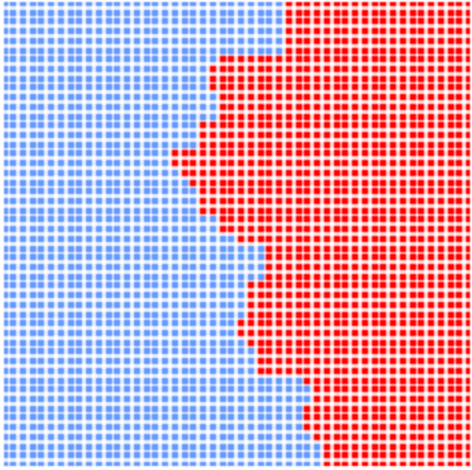
\includegraphics[width=0.215\textwidth]{images/helpful-balancing/1}}
    \caption[short]{początkowy podział}
\end{subfigure}%

\begin{subfigure}{.5\textwidth}
    \centering
    \fbox{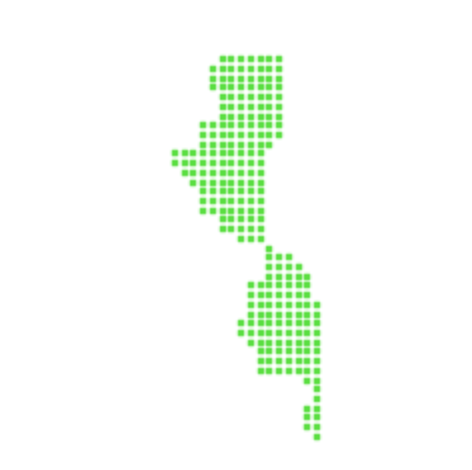
\includegraphics[width=\imgss\textwidth]{images/helpful-balancing/2}}
    \caption[short]{krok 1 - budowanie zbioru helpful}
\end{subfigure}
\begin{subfigure}{.5\textwidth}
    \centering
    \fbox{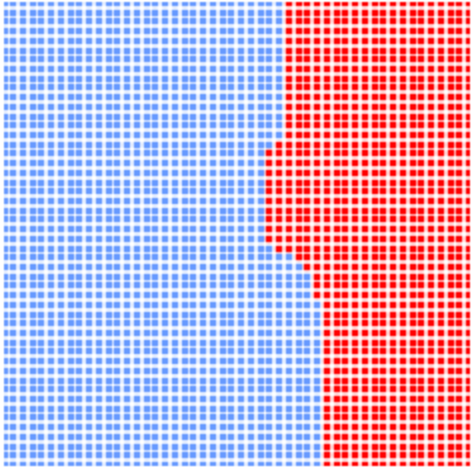
\includegraphics[width=\imgss\textwidth]{images/helpful-balancing/3}}
    \caption[short]{krok 2 - przeniesienie zbioru helpful}
\end{subfigure}%

\begin{subfigure}{.5\textwidth}
    \centering
    \fbox{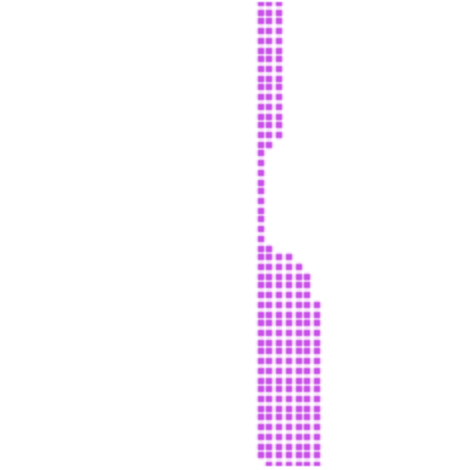
\includegraphics[width=\imgss\textwidth]{images/helpful-balancing/4}}
    \caption[short]{krok 3 - budowanie zbioru balancing}
\end{subfigure}
\begin{subfigure}{.5\textwidth}
    \centering
    \fbox{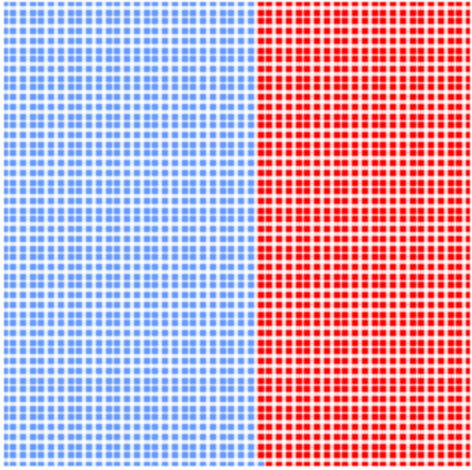
\includegraphics[width=\imgss\textwidth]{images/helpful-balancing/5}}
    \caption[short]{krok 4 - przeniesienie zbioru balancing}
\end{subfigure}%
\caption{Obrazki pokazują początkowy podział, a następnie jedno wywołanie algorytmu Helpful Sets. Rozmiar partycji pozostaje
niemal identyczny, zmniejsza się długość granicy.}
\label{im:balancing}
\end{figure}

\newpage

\begin{pseudocode}
@\underline{HelpfulSet$(A,B)$}@
  IF cut_size$_{A-B}$ $<$ $0$
    RETURN;
  ENDIF
  $l_A \leftarrow l_B \leftarrow cut/2$;                        /* Initialize the limits */
  $s_{max} = (|A| + |B|) / 2) \cdot 0.2$;                /* Initialize max size of HS */
  WHILE $l_A + l_B \geq 1$
    IF $l_A = 0$ OR $2 \cdot l_A \leq l_B$  /* Choose the more promising partition */
      Swap$(A,B)$;
    $S_A$ $=$ BuildHS$(A, l_A, s_{max})$;
    ENDIF
    IF $h(S_A) \leq l_A$ /* If the helpfulness of $S_A$ is smaller than wanted ...
      $l_A \leftarrow b(S_A)$;          ... adjust the limit for the next search */
      IF $l_B > h(S_A)$
        $S_B$ $=$ BuildHS$(B, l_B, s_{max})$;
        IF $h(S_B) \geq h(S_A)$ /* Name the partition with the better set A ...
          Swap$(A, B)$;
        ELSE
          $l_B \leftarrow b(S_B)$; ... and reduce the limit of the other partition */
        ENDIF
      ENDIF
      UndoBuild$(S_B)$;
    ENDIF
    IF $len(S_A) == 0$
      $l_A = 0$;
      CONTINUE;
    ENDIF
    $l_A \leftarrow min(l_A,h(S_A))$;          /* Adjust the limit for the next search */
    MoveSet$(S_A)$                             /* Move the helpful set */
    $min, max$ $\leftarrow$ DetermineMaxAndMin$(w(S_A))$;
    $S_B$ $=$ BuildBS$(B,1 - h(S_A),min,max)$;
    IF $w_l \leq w(S_B) \leq w_h$ and $h(S_B) > -h(S_A)$  /* Check, if the BS is ok */
      MoveSet$(S_B)$;                       /* Yes: Move the BS */
      $l_A \leftarrow l_A + \log(l_A)$;                  /* Increase the limits */
      $l_B \leftarrow l_B + 1$;
    ELSE
      UndoBuild$(S_B)$;           /* No: Undo the build operation and
      UndoMove$(S_A)$;              the movement of the helpful set */
      $l_A \leftarrow l_A/4$;                            /* Reduce the limits */
      $l_B \leftarrow l_B/2$;
    ENDIF
  ENDWHILE
  IF cut_size$_{A-B}$ $>$ $0.1$ $\cdot$ longer_edge_of_a_grid
    Balance$(A, B)$;
  ENDIF
\end{pseudocode}
\vspace{-8mm}
\captionof{listing}{Kod przedstawiający zmodyfikowany na potrzeby niniejszej pracy algorytm Helpful-Set $2$-partitioning.}
\label{code:helpful_sets}
\newpage
Kluczowym elementem algorytmu jest ustalenie wartości helpfulness $l$ zbiorów, których szukamy.
Jeśli wartość $l$ jest zbyt mała, to obiecujące zbiory są przeoczane, natomiast jeśli $l$ jest za duże,
to czas wykonywania algorytmu jest dłuższy, natomiast znalezione przy tym zbiory nie są lepsze.
W celu uzyskania $l$, Party używa techniki zwanej \texttt{adaptive limitation} \cite{article}.
Początkowe $l$ ustawiane jest na wartość $cut/2$.
Wartość $l$ jest zmniejszana o połowę albo ustawiana na najlepszą znalezioną wartość helpfulness, jeśli zbiór $l$-helpful
nie może zostać znaleziony w żadnym z dwóch optymalizowanych zbiorów oraz podwajana, jeśli poszukiwanie
zakończy się sukcesem.
Autorzy \cite{1364754} zaproponowali kilka modyfikacji do algorytmu.
Po pierwsze, zamiast używać pojedynczego limitu $l$ użyto dwóch oddzielnych limitów dla zbioru $A$ oraz zbioru $B$.
Po drugie, dopuszczono do pojawiania się małych różnic wielkości obszarów.
Jest to szczególnie ważne, kiedy podział optymalizowany jest wielokrotnie, na niecałkowicie przywróconym
do początkowego rozmiaru grafie.
Przenoszone wówczas wierzchołki mają często wagi $\geq 1$, ponadto istnieją różnice pomiędzy wagami wierzchołków,
co przekłada się na trudności w idealnym zbalansowaniu optymalizowanych obszarów.
To podejście zostało również zaimplementowane w bibliotekach Jostle and Metis.
Udowodniono, że wpływa ono pozytywnie na optymalizację długości granic, ponieważ dopuszczenie niewielkich
różnic w powierzchni pól pozwala zwykle na lepsze zoptymalizowanie długości granic.
Po trzecie algorytm balansowania obszarów, który zachłannie wyrównuje pola obszarów został przeniesiony na koniec.

Algorytm \ref{code:helpful_sets} przedstawia zmodyfikowaną przeze mnie procedurę.
Pierwszą moją modyfikacją jest sprawdzanie, czy balansowane obszary wciąż ze sobą graniczą (linia $2$).
Może się zdarzyć, że na skutek balansowania innych obszarów granica ta zostanie przerwana.
Jak w poprzedniej implementacji, limity $l_A$ oraz $l_B$ ustawiane są na połowę aktualnej długości granicy pomiędzy
obszarami $A$ i $B$ (linia $5$).
W rozwiązaniu zaproponowanym przez autorów \cite{1364754}, podczas wyszukiwania, wartość helpful zbioru helpful nie może stać się mniejsza
niż $-d/2$, nie może również przekroczyć wagi $s_{max}$.
Wartość $d$ to średni stopień wierzchołka w grafie.
Dla mojej implementacji mógłbym założyć, że $d$ jest zawsze równe $4$ - wynika to ze sposobu, w jaki buduję
graf z wejściowej siatki (rysunek \ref{im:indivisible}).
Jednak ta zasada nie działa.
Algorytm budowania zbioru helpful jest bowiem zachłanny i często budował zbiory, które spełniały kryterium nieprzekraczania
wagi $s_{max}$ oraz miały ujemną wartość helpful, większą niż $-2$.
Jednak później w kodzie oryginalnego algorytmu sprawdzane było, czy zbiór nie ma ujemnej wartości helpful i
jeśli miał to budowanie zaczynało się od początku.
Przez to algorytm wywoływał się wielokrotnie bez zakończenia się sukcesem.
Moim rozwiązaniem była zmiana tej instrukcji na warunek na wielkość zbioru $S_A$ (linia $25$) oraz na
pozwolenie na budowanie zbiorów o wartości helpful większej bądź równej $0$ (linia $11$ oraz $16$).
$s_{max}$ z kolei, autorzy \cite{article} ustawiali na wartość $128$.
Ja uzależniłem $s_{max}$ od rozmiaru optymalizowanych partycji (linia $6$).
Użyty do tego współczynnik $0.2$ może zostać dowolnie zmieniony.
Jednak wedle mojego doświadczenia powinien być on raczej mniejszy niż $0.4$, aby zbiór helpful nie był zbyt duży.
Zwiększa to czas partycjonowania, ale nie poprawia wyników.
Lepiej by był on nieco za mały niż za duży, ponieważ po udanych znalezieniu małego zbioru helpful oraz zbioru balancig
limit i tak zostanie zwiększony, a zaczynanie od bardzo dużego zbioru helpful często kończy się nieudanym poszukiwaniem
zbioru balancing i powrotem do początkowego podziału.
Poszukiwanie dużego zbioru jest bardziej kosztowne.

\newpage
\begin{figure}[h]
\begin{subfigure}{\textwidth}
    \centering
    \fbox{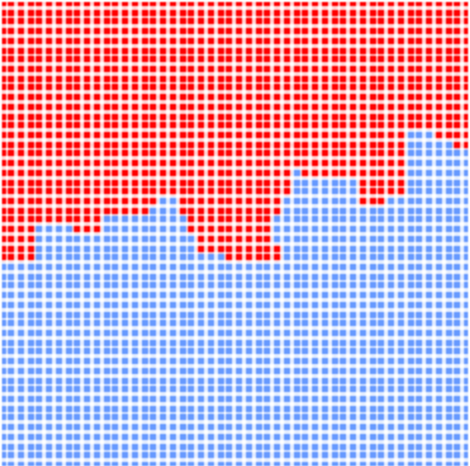
\includegraphics[width=0.215\textwidth]{images/helpfulsets-sh/0}}
    \caption[short]{początkowy podział}
\end{subfigure}%

\begin{subfigure}{.5\textwidth}
    \centering
    \fbox{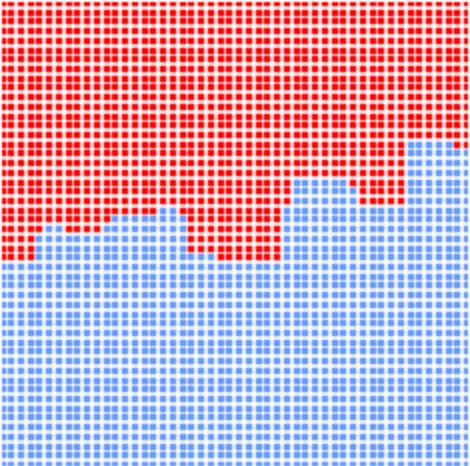
\includegraphics[width=\imgss\textwidth]{images/helpfulsets-sh/1}}
    \caption[short]{krok 1 - przeniesienie zbioru helpful}
\end{subfigure}
\begin{subfigure}{.5\textwidth}
    \centering
    \fbox{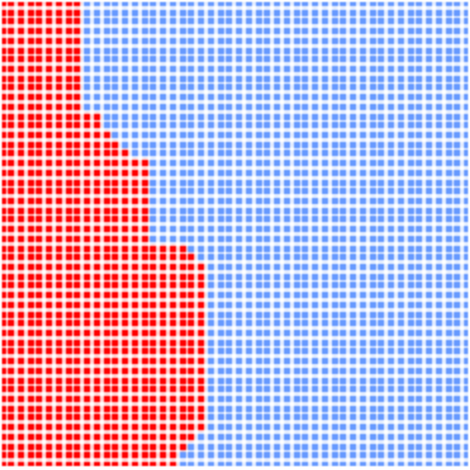
\includegraphics[width=\imgss\textwidth]{images/helpfulsets-sh/2}}
    \caption[short]{krok 2 - przeniesienie zbioru balancing}
\end{subfigure}%

\begin{subfigure}{.5\textwidth}
    \centering
    \fbox{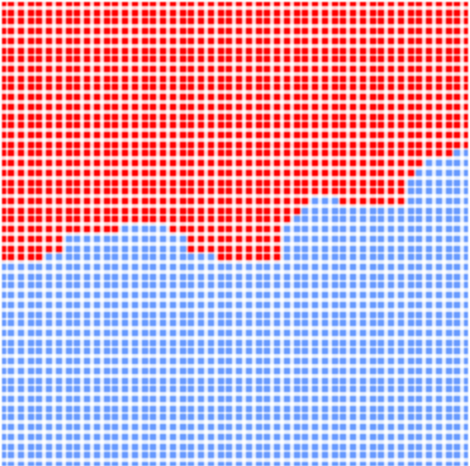
\includegraphics[width=\imgss\textwidth]{images/helpfulsets-sh/3}}
    \caption[short]{krok 3 - przeniesienie zbioru helpful}
\end{subfigure}
\begin{subfigure}{.5\textwidth}
    \centering
    \fbox{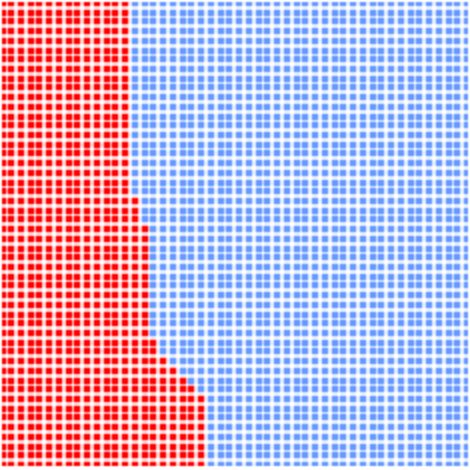
\includegraphics[width=\imgss\textwidth]{images/helpfulsets-sh/4}}
    \caption[short]{krok 4 - przeniesienie zbioru balancing}
\end{subfigure}%

\begin{subfigure}{.5\textwidth}
    \centering
    \fbox{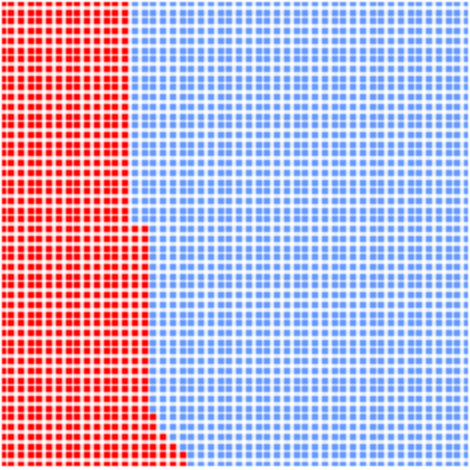
\includegraphics[width=\imgss\textwidth]{images/helpfulsets-sh/5}}
    \caption[short]{krok 5 - przeniesienie zbioru helpful}
\end{subfigure}
\begin{subfigure}{.5\textwidth}
    \centering
    \fbox{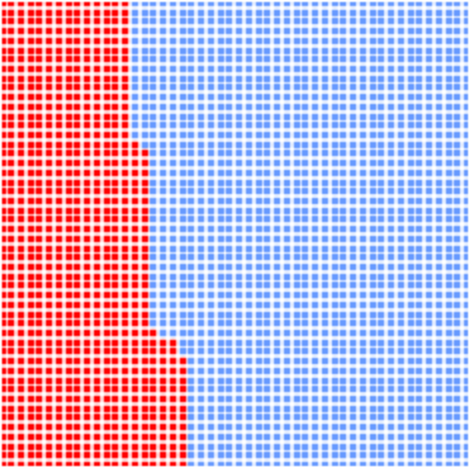
\includegraphics[width=\imgss\textwidth]{images/helpfulsets-sh/6}}
    \caption[short]{krok 6 - przeniesienie zbioru balancing}
\end{subfigure}%

\begin{subfigure}{.5\textwidth}
    \centering
    \fbox{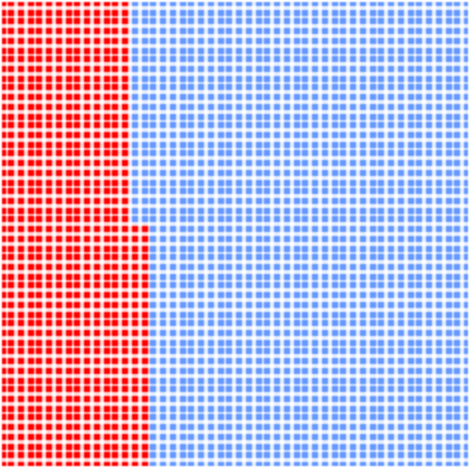
\includegraphics[width=\imgss\textwidth]{images/helpfulsets-sh/7}}
    \caption[short]{krok 7 - przeniesienie zbioru helpful}
\end{subfigure}
\begin{subfigure}{.5\textwidth}
    \centering
    \fbox{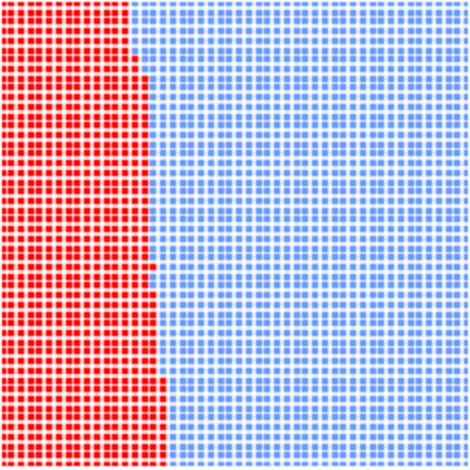
\includegraphics[width=\imgss\textwidth]{images/helpfulsets-sh/8}}
    \caption[short]{krok 8 - przeniesienie zbioru balancing}
\end{subfigure}
\caption{Obrazki przedstawiają kolejne kroki działania algorytmu Helpful Sets na siatce 50x50 podzielonej na 2 obszary
przez algorytm LAM. W pierszym kroku tworzony jest stosunkowo mały zbiór helpful, a w kolejnym kroku odpowiednio mały zbiór balancing.
W momencie kiedy to się udaje algorytm zwiększa limit liczby wierzchołków, dlatego kolejne kroki wnoszą więcej zmian.
Po 4 cyklach budowania i przenoszenia zbioru helpful oraz zbioru balancing granica między obszarami jest znacząco mniejsza, a wielkość obszarów
zachowana. Na potrzeby przykładu balansowanie pól jest wyłączone.}
\label{im:h_steps}
\end{figure}
\FloatBarrier

Pętla WHILE, która znajduje się między liniami $7$ i $42$ jest wykonywana, dopóki suma limitów jest większa od $1$.
W oryginalnej implementacji było to $0$, jednak wedle mojego doświadczenia algorytm wywoływał się wtedy bardzo długo,
niekoniecznie zwiększając jakość partycjonowania.
Jeśli zbiór $l_A$-helpful ($S_A$) (z wagą $w(S_A)$ oraz wartością helpfulness wynoszącą $h(S_A)$) nie może zostać
znaleziony (linia $12$), limit jest redukowany to najlepszej znalezionej wartości helpfulness ($b(S_A)$).
Dalej podejmowana jest decyzja czy nastąpi wyszukiwanie w partycji $B$ (linia $14$).
Jeśli limit $l_A$ jest dużo mniejszy od limitu $l_B$ zbiory $A$ i $B$ są ze sobą zamieniane.
Ten warunek powoduje, że zbiór helpful szukany jest najpierw w bardziej obiecującej partycji.
Jeśli tak, to ustalany jest zbiór $S_B$ (linia $15$).
Dalej zbiór z większą wartością helpfulness jest nazywany $S_A$ (linia $17$) lub limit
drugiej partycji jest redukowany (linia $19$), a zbiór $S_B$ usuwany (linia $22$).
Jeśli wielkość zbioru helpful jest równa $0$, to limit ustawiany jest na $0$ (linia $25$), a algorytm powtarzany.
W przeciwnym wypadku do $l_A$ przypisywana jest nowa wartość (linia $28$), $S_A$ przenoszone jest do $B$ (linia $29$),
a wywołanie wkracza w fazę szukania zbioru balancing.
W tym celu obliczany jest przedział $[min, max]$ dla zbioru balancing (linia $30$).
W implementacji zaproponowanej w \cite{1364754} wartości $min$ oraz $max$ były obliczane w następujący sposób:
\vspace{-3mm}
\begin{pseudocode}
$min \leftarrow (w(B) - w_{max}(B) - grace)^+$
$max \leftarrow (w(B) - w_{min}(B) + grace)^+$
\end{pseudocode}
\vspace{-13mm}
\captionof{listing}{}
\label{code:old_min_max}
\vspace{3mm}
gdzie $grace$ jest połową wagi najcięższego wierzchołka.
Jednak ten sposób wyznaczania wartości $min$ oraz $max$ nie sprawdzał się w moich testach.
$max$ i $min$ pozwalają na budowanie zbioru balancing o przedziale wag $[min, max]$.
Rzadko jednak algorytm nie był w stanie osiągnąć wartości $max$.
Najczęściej była to wartość bliska lub równa $max$.
Ponadto na początku algorytmu znajduje się kod odpowiedzialny za wybieranie lepszego zbioru do budowania zbioru helpful.
Testy pokazały, że podczas wielokrotnych wywołań, pomimo ciągłych wymian wierzchołków między obszarami,
zwykle to ten sam obszar jest wybierany jako ten lepszy do budowania zbioru helpful.
W efekcie jeśli zbiór balancing był za każdym razem bliski $max$ (czyli był nieco większy od zbioru helpful) oraz
był on budowany na tym samym obszarze, to jeden obszar sukcesywnie rósł kosztem drugiego.
W związku z tym zaproponowałem poniższe rozwiązanie, które losowo decyduje, czy wartość $max$ ma być trochę mniejsza, czy
trochę większa od zbioru helpful:
\vspace{-3mm}
\begin{pseudocode}
@\underline{DetermineMaxAndMin$(w(S_A))$}@
  $rand$ $=$ RandValue$(0,1)$   /* draws either $0$ or $1$ */
  IF $rand$ $==$ $1$
    $min$ $=$ $| w(S_A) - 0.1 \cdot w(S_A) |$
    $max$ $=$ $| w(S_A) + 0.1 \cdot w(S_A) |$
  ELSE
    $min$ $=$ $| w(S_A) - 0.2 \cdot w(S_A) |$
    $max$ $=$ $| w(S_A) - 0.1 \cdot w(S_A) |$
  ENDIF
  RETURN $min$, $max$
\end{pseudocode}
\vspace{-13mm}
\captionof{listing}{}
\label{code:new_min_max}
\FloatBarrier

Za pomocą tych granic algorytm wyszukuje zbiór balancing $S_B$, który nie zwiększy długości granicy pomiędzy $A$ i $B$
o więcej niż $1 - h(S_A)$ (linia $31$).
Jeśli szukanie takiego zbioru zakończy się sukcesem, to jest on przenoszony do zbioru $A$ i limity dla obydwu zbiorów
($l_A$ oraz $l_B$) są zwiększane (linie $33$-$35$).
W przeciwnym wypadku $S_B$ jest usuwany, $S_A$ przenoszone z powrotem do $A$, a limity $l_A$ oraz $l_B$ zmniejszane
(linie $37$-$40$).
Jeśli algorytm nie może już poprawiać więcej partycjonowania sprawdzany i w razie potrzeby poprawiany jest balans pól
(linia $43$).
Dodatkową modyfikacją wprowadzoną przeze mnie był warunek na uruchomienie procedury 'Balance', który jest omawiany
dokładniej w dalszych częściach pracy.
Jego celem jest uniemożliwienie balansowania pól między obszarami o bardzo krótkiej granicy.

\newpage
\subsubsection{Szczegóły budowania zbioru helpful}
Główna funkcja tej heurystyki działa podobnie do algorytmu Kruskala do wyliczania
najmniejszego drzewa rozpinającego \cite{algorithms222}.
Startuje od pustego zbioru (o wartości helpfulness równej $0$) i buduje go za pomocą wierzchołków z jednej strony granicy.
W każdym kroku wybiera wierzchołek z wartością helpfulness z pewnego przedziału, przenosi go do zbioru
(helpfulness zbioru zwiększa się wtedy o helpfulness wierzchołka), następnie zwiększa wartość helpfulness wierzchołków,
które są w tej samej partycji i są sąsiednie do przeniesionego wierzchołka,
Te wierzchołki zyskują jedną krawędź zewnętrzną
kosztem jednej krawędzi wewnętrznej, w związku z powyższym ich wartość helpfulness rośnie o $2$.
\begin{figure}[h]
    \centering
    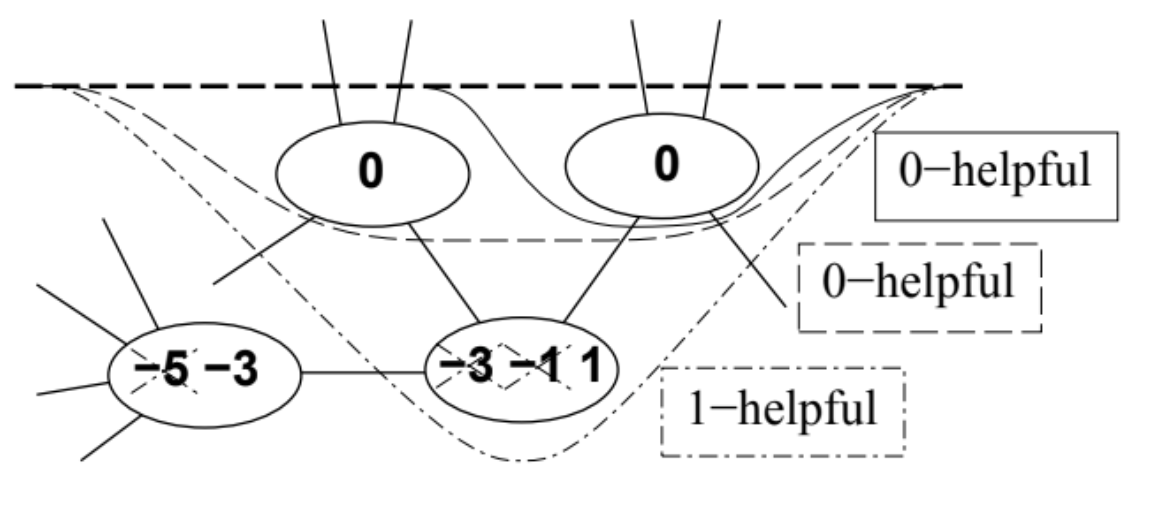
\includegraphics[width=0.6\linewidth]{images/changing_helpful_values}
    \caption{Zmiana wartości helpfulness dla sąsiadów.
    Źródło: \cite{article}.}
    \label{im:helpfulness_neighbours}
\end{figure}

Branie pod uwagę tylko wierzchołków z jednej strony granicy pozwala na budowanie zbioru z dwóch stron podziału jednocześnie.
Jeśli znaleziony zbiór wierzchołków jest przemieszczany między partycjami, to wartości helpfulness dla wierzchołków
docelowej partycji muszą również zostać zaktualizowane.
Podczas budowania zbioru jego wielkość zwiększa się w każdym kroku.
Zbiór helpful przestaje być budowany w następujących przypadkach:
\begin{itemize}
    \item wartość helpfulness dla zbioru osiągnie wartość limitu,
    \item {brane są pod uwagę tylko wierzchołki o pewnej wartości helpfulness, a te się skończą,}
    \item wielkość zbioru osiągnie wartość limitu.
\end{itemize}
Ważną obserwacją jest fakt, że jeśli brane pod uwagę są jedynie wierzchołki z wartością helpfulness $\geq$ $0$,
to helpfulness zbioru albo zachowuje tę samą wartość, albo rośnie, ale nigdy nie maleje.
Podobieństwo tego algorytmu do algorytmu BFS objawia się w sposobie, w jakim wierzchołki przypisywane są do zbioru.
Wierzchołek może zostać wybrany, jeśli jego wartość helpfulness jest większa od ustalonej wartości.
To następuje albo jeśli wierzchołek ma od początku odpowiednią wartość helpfulness, albo jeśli urośnie ona do odpowiedniej
wartości podczas budowania zbioru (poprzez dodanie do zbioru jego sąsiadów).

\newpage
\begin{figure}[h]
\begin{subfigure}{.32\textwidth}
    \centering
    \fbox{\includegraphics[width=0.7\textwidth]{images/building-helpfulsets/3}}
    \caption[short]{podział}
\end{subfigure}
\begin{subfigure}{.32\textwidth}
    \centering
    \fbox{\includegraphics[width=0.7\textwidth]{images/building-helpfulsets/4}}
    \caption[short]{wartości helpfulness wierzchołków}
\end{subfigure}
\begin{subfigure}{.32\textwidth}
    \centering
    \fbox{\includegraphics[width=0.7\textwidth]{images/building-helpfulsets/5}}
    \caption[short]{wierzchołki do budowania zbioru helpful}
\end{subfigure}
\caption{Obrazki przedstawiają jak wygląda zbiór wierzchołków, na bazie którego budowany jest zbiór helpful.
Obrazek (a) przedstawia partycjonowanie. Zbiór helpful będzie budowany na niebieskiej partycji.
Obrazek (b) przedstawia wszystkie wierzchołki zbioru (a), gdzie kolor oznacza wartość helpful. Skala rozpoczyna się od
koloru ciemnoniebieskiego dla wierzchołków z wartością helpfulness wynoszącą $-4$ i przechodzi do czerwonego dla wierzchołków z
wartością helpfulness $4$. Widoczna jest większa wartość helpfulness dla wierzchołków przy granicy. Obrazek (c)
przedstawia wierzchołki, które brane są pod uwagę przez algorytm. Są one filtrowanie na etapie budowania zbioru,
tak by zawsze wybierane były wierzchołki znajdujące się na granicy.}
\label{im:building_helpfulsets}
\end{figure}

Dodatkową modyfikacją, którą wprowadziłem, było filtrowanie wierzchołków, tak by algorytm wybierał wierzchołek z największą
wartością helpfulness tylko spośród wierzchołków granicznych.
Została ona zaimplementowana w związku z powstającymi obszarami rozproszonymi
(to negatywne zjawisko opisuje w późniejszych częściach pracy).
Chciałem aby istniała pewność, że wybierany wierzchołek jest zawsze wierzchołkiem granicznym.
Rysunek \ref{im:building_helpfulsets} przedstawia moje rozwiązanie.
\newpage
\subsubsection{Szukanie zbioru $k$-helpful gdzie $k \geq limit$}
Proces budowania zbiorów helpful pokazany jest na rysunku \ref{im:building-helpfulsets}(a).
Te zbiory nazywane są zbiorami Help.
Kardynalność tych zbiorów rośnie dynamicznie podczas szukania.
Dzięki temu, że podczas budowania zbioru Help aktualizujemy tylko wartości helpfulness wierzchołków z tej samej partycji,
obydwa zbiory Help mogą byc budowane niezależnie i równolegle.
Jednak w mojej implementacji (rysunek \ref{code:helpful_sets}) budowane są one jeden po drugim
(jeśli warunek pozwoli na zbudowanie drugiego).

Podczas tego procesu brane pod uwagę są tylko wierzchołki z wartością helpfulness $\geq$ $0$.
Może to prowadzić do przedwczesnego zakończenia wywołania algorytmu, jeśli żadne wierzchołki z taką wartością
helpfulness nie będą już dostępne, ale to także gwarantuje, że wartość helpfulness dla zbioru Help nigdy nie będzie
maleć.
Wyszukiwanie zbioru Help kończy się, gdy jego wartość helpfulness osiąga \texttt{limit} lub jeśli nie ma więcej wierzchołków
z wartością helpfulness $\geq$ $0$.

Po udanym wywołaniu, zbiór $S$, który jest zbiorem Help z większą wartością helpfulness, przenoszony jest
na drugą stronę podziału.
Drugi zbiór Help jest usuwany i nie jest więcej brany pod uwagę.
Na rysunku \ref{im:building-helpfulsets}(b) BIG SET reprezentuje $V_1$ lub $V_2$ połączone z $S$.
SMALL SET to pozostała część, która została zredukowana o $S$.
\begin{figure}[h]
\begin{subfigure}{.5\textwidth}
    \centering
    \includegraphics[width=0.8\textwidth]{images/building-helpfulsets/1}
    \caption[short]{}
\end{subfigure}
\begin{subfigure}{.5\textwidth}
    \centering
    \includegraphics[width=0.8\textwidth]{images/building-helpfulsets/2}
    \caption[short]{}
\end{subfigure}%
\caption{Szukanie zbioru $k$-helpful poprzez przenoszenie wierzchołków z wartością helpfulness $\geq$ $0$
do zbiorów Help (a). (b) to przenoszenie zbioru $S$ na drugą stronę podziału.
Źródło: \cite{article}.}
\label{im:building-helpfulsets}
\end{figure}
\newpage
\subsubsection{Szczegóły budowania zbioru balancing}

Znalezienie zbioru balancing jest trudniejsze, z racji na dodatkowe obostrzenia związane z jego rozmiarem oraz wartością
helpfulness.
Zbiór $\bar{S}$ musi mieć ten sam rozmiar co zbiór $S$ oraz jego wartość helpfuless musi być tak duża jak to możliwe,
lecz nie mniejsza niż $-k+1$-helpful, jeśli $S$ był $k$-helpful.
Idea budowania zbioru balancing polega na rozpoczęciu od pustego zbioru $\bar{S}$ i wybraniu podzbioru
ze zbioru BIG SET, który zwiększy jego rozmiar tak bardzo jak to możliwe oraz jednocześnie zmniejszy jego wartość
helpfulness tak mało jak to możliwe.
Algorytm podzielony jest na trzy fazy.
Pierwsza faza dodaje do zbioru wierzchołki, których wartości helpfulness są $\geq$ $0$.
Druga faza próbuje znaleźć podzbiory wierzchołków, które dodane do $\bar{S}$, pozostawią jego helpfulness na jednym
poziomie - szuka zbiorów $0$-helpful.
Każda z tych faz kończy swoje wywołanie jeśli $\bar{S}$ jest wystarczająco duży.
Jeśli dwie pierwsze fazy są niewystarczające, uruchamiana jest trzecia faza, która oparta jest na zachłannym dobieraniu
wierzchołków, w celu dokończenia budowania zbioru balancing.

\begin{figure}[h]
\begin{subfigure}{.32\textwidth}
    \centering
    \fbox{\includegraphics[width=0.7\textwidth]{images/helpful-balancing/3}}
    \caption[short]{podział}
\end{subfigure}
\begin{subfigure}{.32\textwidth}
    \centering
    \fbox{\includegraphics[width=0.7\textwidth]{images/helpful-balancing/6}}
    \caption[short]{faza 1}
\end{subfigure}
\begin{subfigure}{.32\textwidth}
    \centering
    \fbox{\includegraphics[width=0.7\textwidth]{images/helpful-balancing/4}}
    \caption[short]{faza 2}
\end{subfigure}
\caption{Obrazki przedstawiają fazę pierwszą oraz fazę drugą budowania zbioru balancing.
Ten sam przypadek podziału można znaleźć na rysunku \ref{im:balancing}.}
\label{im:balancing:details}
\end{figure}

\textbf{Faza 1}

Pierwsza faza jest najmniej skomplikowana.
Dopóki w zbiorze BIG SET są wierzchołki z wartościami helpfulness $\geq$ $0$, wierzchołek z największą wartością
helpfulness dodawany jest do zbioru $\bar{S}$.
Te wierzchołki uznawane są jako wierzchołki, które należą już do drugiej partycji, więc wartości helpfulness
ich sąsiadów z poprzedniej partycji muszą wzrosnąć o 2.
Podczas tej fazy wielkość $\bar{S}$ wzrasta, a wartość $H(\bar{S})$ pozostaje taka sama lub się powiększa.
Faza pierwsza kończy się jeśli utworzony zostanie zakładany zbiór balancing lub nie ma więcej wierzchołków
w zbiorze BIG SET, których wartości helpfulness są przynajmniej równe $0$.

\vspace{8mm}
\textbf{Faza 2}

Ta faza próbuje znaleźć zbiory $0$-helpful, to znaczy podzbiory zbioru BIG SET, które przeniesione do $\bar{S}$,
nie zmniejszą jego wartości helpfulness.
Koncepcja tej fazy polega na przeprowadzeniu kilku wyszukiwań, rozpoczynając od pojedynczego wierzchołka
$-1$-helpful lub $-2$-helpful.
Każde z wyszukiwań próbuje dopełnić swój podzbiór wierzchołków do zbioru $0$-helpful.
Ważną obserwacją jest, że na początku tego etapu BIG SET nie zawiera żadnych wierzchołków z wartością
helpfulness większą bądź równą zero.

\begin{figure}[h]
    \centering
    \includegraphics[width=0.95\linewidth]{images/0-helpful-sets}
    \caption{Przykłady zbiorów 0-helpful. Źródło: \cite{article}.}
    \label{im:0-helpful}
\end{figure}

Rysunek \ref{im:0-helpful} pokazuje przykładowe zbiory $0$-helpful.
Nie ma jednego przepisu na zbiór $0$-helpful, mogą być to różne konstrukcje wierzchołków, a intencją drugiej fazy
jest znalezienie jak największej liczby tego typu zbiorów.

Rysunek \ref{im:phase_2} pokazuje drugą fazę.
Tak jak w fazie pierwszej, wykorzystywana jest ta sama metoda budowania zbioru (sekcja $4.1.6$).
Jednak zamiast przenosić wierzchołki bezpośrednio do $\bar{S}$, są one przechowywane w zbiorze o nazwie $-2$-SET.
$-2$-SET zawiera aktualny podzbiór wierzchołków, który faza druga próbuje dopełnić do zbioru $0$-helpful.
Niech $k' = k + H(\bar{S})$ będzie poprawą długości granicy, spowodowaną przez przeniesienie $S$ i $\bar{S}$, każdy
na odpowiednią stronę podziału.
Na początku każdego poszukiwania zbioru $-2$-SET rozpatrywane są jedynie wierzchołki z wartością helpfulness, wynoszącą
$max(-2, -k'+1)$.
Następnie tylko wierzchołki, które są przynajmniej $0$-helpful mogę być umieszczone w zbiorze $-2$-SET.
To gwarantuje, że dowolny $-2$-SET może zostać przeniesiony do $\bar{S}$ na każdym etapie algorytmu, bez znaczącego
zmniejszania jego wartości helpfulness.
Jest to szczególnie istotne jeśli $-2$-SET jest wystarczająco duży, aby zakończyć balansowanie.
Podsumowując:
\begin{itemize}
    \item {tylko wierzchołki $-1$-helpful oraz $-2$-helpful ze zbioru BIG SET są rozważane na początku budowania $-2$-SET,}
    \item wartość helpfulness zbioru $-2$-SET jest co najmniej równa $-2$ i nigdy nie maleje,
    \item jeśli $k'$ wynosi $2$ tylko wierzchołki $-1$-helpful mogą zostać wybrane oraz
    \item jeśli $k'$ wynosi $1$ faza druga w ogóle się nie rozpoczyna.
\end{itemize}

Jeśli wyszukiwanie zbioru $-2$-SET zakończy się i jego wartość helpfulness jest mniejsza od $0$ to jest przechowywany
do dalszego użycia.
\begin{figure}[h]
    \centering
    \includegraphics[width=0.65\linewidth]{images/phase2}
    \caption{Obrazek przedstawiający fazę 2. Źródło: \cite{article}.}
    \label{im:phase_2}
\end{figure}
\newpage

\begin{pseudocode}
@\underline{PROCEDURE Phase 2}@
  WHILE $(|\bar{S}| < |S|)$ AND BIG SET contains nodes with helpfulness $\geq$ $max(-2, -k + 1 - H(\bar{S})$
    start building a $-2$-SET with the max. helpful node;

    WHILE H$(-2$-SET$)$ $<$ $0$ AND $(|-2$-SET$|$ + $|\bar{S}|$ $<$ $|S|)$ AND
          BIG SET has node with helpfulness $\geq$ $0$
      move node with the highest helpfulness to $-2$-SET;
    ENDWHILE

    IF H$(-2$-SET$)$ $\geq$ 0
      move $-2$-SET to $\bar{S}$;
      WHILE $(|\bar{S}|$ $<$ $|S|)$ AND $-2$-COLL contains sets $S'$ with H$(S')$ $\geq$ $0$
        take set $S'$ $\in$ $-2$-COLL with max. helpfulness;
        IF $|S'|$ + $|\bar{S}|$ $<$ $|S|$
          move $S'$ to $\bar{S}$;
        ELSE
          reduce $S'$ to $|S|$ - $|\bar{S}|$ and move it to $|\bar{S}|$;
        ENDIF
    ELSE IF $| -2$-SET$|$ + $|\bar{S}|$ = $|S|$
      move $-2$-SET to $\bar{S}$;
    ELSE
      move $-2$-SET to $-2$-COLL;
    ENDIF
  ENDWHILE
\end{pseudocode}
\vspace{-8mm}
\captionof{listing}{Algorytm przedstawiający fazę drugą. Źródło: \cite{article}.}
\label{code:phase_2}
\vspace{4mm}
Kolekcja zbiorów $-2$-SET jest nazywana $-2$-COLL.
Zawiera ona podzbiory wierzchołków, które są co najmniej $-2$-helpful.
Wiele z nich może zostać zbiorami $0$-helpful, jeśli inne zbiory $-2$-SET zostaną przeniesione do $\bar{S}$.
Aktualizacja wartości helpfulness sąsiadów podczas budowania zbioru $-2$-SET następuje tylko dla wierzchołków,
które są częścią zbioru BIG SET.
Zbiory $-2$-SET będące w zbiorze $-2$-COLL nie są uznawane za zbiory, które zmieniły stronę partycjonowania.
W związku z tym, jeśli $-2$-SET nie może zostać uzupełniony wierzchołkami, aby być $0$-helpful i jest przenoszony
do zbioru $-2$-COLL, to wartości helpfulness wierzchołków w zbiorze BIG SET, które były jego sąsiadami, są przywracane
do poprzednich wartości.
Na tym etapie algorytmu podczas budowania zbioru $-2$-SET, wartości helpfulness sąsiednich wierzchołków w zbiorze
$-2$-COLL nie są zmieniane, ponieważ wierzchołki w zbiorze $-2$-COLL nie są brane pod uwagę przy budowaniu zbiorów
$-2$-SET.
Tylko jeśli zbiór $-2$-SET zostanie $0$-helpful i jest przenoszony do $\bar{S}$ to aktualizowane są wartości helpfulness
jego sąsiadów będących w zbiorze $-2$-COLL.

Algorytm \ref{code:phase_2} przedstawia fazę drugą.
Szukanie zbioru $-2$-SET kończy się w następujących przypadkach:
\begin{enumerate}
    \item {Wartość helpfulness zbioru $-2$-SET staje się większa bądź równa 0. W tym przypadku cały zbiór $-2$-SET
    przenoszony jest do zbioru $\bar{S}$. Wartości helpfulness sąsiednich wierzchołków znajdujących się w zbiorze
    $-2$-COLL są aktualizowane. Każda taka aktualizacja wartości helpfulness dla wierzchołka w zbiorze $-2$-COLL
    skutkuje tym, że wartość helpfulness jednego znajdującego się tam zbioru $-2$-SET podnosi się o 2. W związku z tym
    wiele z nich może zostać co najmniej $0$-helpful, a następnie zostać przeniesione do $\bar{S}$.
    Algorytm wybiera zawsze zbiór $-2$-SET z największą wartością helpfulness i przenosi go do $\bar{S}$, tak długo
    jak w $-2$-COLL są takie zbiory.

    Jeśli, któryś z tych zbiorów jest większy niż $|S| - |\bar{S}|$ to jest redukowany do odpowiedniego rozmiaru, poprzez
    usuwanie ostatnio dodanych elementów. Rezultatem takiej redukcji jest $|\bar{S}| = |S|$ oraz zakończenie
    wykonania procedury.}
    \item {Partycja osiąga odpowiedni rozmiar, to znaczy $|-2$-SET$|$ $+$ $|\bar{S}|$ $=$ $|S|$. W tym przypadku wartość
    helpfulness zbioru $-2$-SET wciąż wynosi co najmniej $max(-2, -k' + 1)$ (co jest zagwarantowane procesem jego budowania)
    i może on zostać przeniesiony do zbioru $\bar{S}$. Partycja osiąga w tym wypadku odpowiedni rozmiar i następuje
    zakończenie procedury.}
    \item {Nie ma więcej wierzchołków w zbiorze BIG SET z wartością helpfulness większą bądź równą $0$. W tym wypadku
    aktualnie budowany $-2$-SET nie może zostać powiększony o kolejne wierzchołki, w związku z tym jest przenoszony do
    zbioru $-2$-COLL, gdzie oczekuje na późniejsze wykorzystanie.}
\end{enumerate}

\vspace{8mm}
\textbf{Faza 3}

Ta faza wybiera wierzchołki ze zbioru BIG SET oraz zbiory $-2$-SET ze zbioru $-2$-COLL w celu przeniesienia do
$\bar{S}$.
Wybiera wierzchołek lub zbiór z największą wartością helpfulness tak długo, aż przeniesienie go nie obniży wartości
helpfulness zbioru $\bar{S}$ poniżej wartości $-k+1$.
Jeśli jakiś zbiór $-2$-SET ze zbioru $-2$-COLL jest użyteczny, ale jego rozmiar jest większy niż $|S| - |\bar{S}|$,
to jego rozmiar jest redukowany.
Faza $3$ kończy swoje wywołanie, jeśli przeniesienie jakiegokolwiek zbioru $-2$-SET lub wierzchołka, spowoduje
obniżenie wartości helpfulness zbioru $\bar{S}$ poniżej $-k+1$ lub jeśli uda się wypełnić zbiór $\bar{S}$ do
rozmiaru zbioru $S$.

\newpage
\subsubsection{Balansowanie rozmiarów obszarów}
Ten etap algorytmu wywoływany jest zawsze po procedurze optymalizacji długości granic.
Odpowiedzialny jest za wyrównaniu wielkości pól, które nie są idealnie równe po
wywołaniu algorytmu LAM.
Przez autorów artykułu \cite{1364754} został określony jako algorytm zachłanny, lecz nie opisano szczegółów jego działania.

W związku z powyższym zaimplementowałem następujące rozwiązanie:
algorytm korzysta również z mechanizmu do budowania zbiorów helpful i balancing, to jest z obliczania wartości
helpfulness dla wierzchołków.
Zachłannie wybierane są wierzchołki z największą wartością helpfulness, dopóki pola obszarów nie zostaną
zbalansowane do oczekiwanej wartości różnicy wielkości pól.
Obszary balansują się zabierając wierzchołki obszarów sąsiednich.
Oznacza to, że jeśli wywoływany jest algorytm optymalizacji granic między obszarami $A$ oraz $B$, gdzie obszar $A$
jest większy od obszaru $B$, to po wyrównaniu wielkości pól obszar $A$ odda część wierzchołków obszarowi $B$.

\vspace{4mm}
\begin{figure}[h]
\begin{subfigure}{.5\textwidth}
    \centering
    \fbox{\includegraphics[width=\imgss\textwidth]{images/fields-balacing/1}}
    \caption[short]{krok 1}
\end{subfigure}
\begin{subfigure}{.5\textwidth}
    \centering
    \fbox{\includegraphics[width=\imgss\textwidth]{images/fields-balacing/2}}
    \caption[short]{krok 2}
\end{subfigure}%

\begin{subfigure}{.5\textwidth}
    \centering
    \fbox{\includegraphics[width=\imgss\textwidth]{images/fields-balacing/3}}
    \caption[short]{krok 3}
\end{subfigure}
\begin{subfigure}{.5\textwidth}
    \centering
    \fbox{\includegraphics[width=\imgss\textwidth]{images/fields-balacing/4}}
    \caption[short]{krok 4}
\end{subfigure}%

\begin{subfigure}{.5\textwidth}
    \centering
    \fbox{\includegraphics[width=\imgss\textwidth]{images/fields-balacing/5}}
    \caption[short]{krok 5}
\end{subfigure}
\begin{subfigure}{.5\textwidth}
    \centering
    \fbox{\includegraphics[width=\imgss\textwidth]{images/fields-balacing/6}}
    \caption[short]{krok 6}
\end{subfigure}%
\caption{Obrazki pokazują działania algorytmu optymalizacji granic oraz balansowania rozmiarów pól. Jak widać, z wywołania
na wywołanie, czerwony obszar, który był na początku najmniejszy, stopniowo rośnie odbierając wierzchołki sąsiednim
obszarom. $p$ wynosi $0.1$.}
\label{im:fields_balancing}
\end{figure}

\newpage
Dla działania algorytmu ustalany jest współczynnik $p$, który decyduje o tym ile wierzchołków zostanie wymienionych.
$p$ osiąga wartości od $0$ do $0.5$ i oznacza jaka część różnicy pól balansowanych obszarów będzie przeniesiona do mniejszego obszaru.
$V_b$ to wierzchołki wytypowane przez algorytm balansowania pól, które zostaną przeniesione do mniejszego
obszaru.
\begin{equation}
|V_b| = p \cdot ||A| - |B||
\end{equation}

Im $p$ będzie mniejsze, tym małe obszary będą rosły wolniej, stopniowo rozbudowując się w kierunku wszystkich sąsiadów.
Im $p$ będzie większe tym proces będzie bardziej gwałtowny, co może bardziej naruszyć podział, na przykład przemieszczając
obszar w jakimś kierunku.
Im $p$ mniejsze, tym więcej wywołań algorytmu optymalizacji jest potrzebne, aby zrównać wielkości pól obszarów.
Zgodnie z moimi obserwacjami, dla współczynników decydujących o częstotliwości
wywołań algorytmu do optymalizacji granic (algorytm \ref{code:main_impr_procedure}), dobrze sprawdza się $p$ wynoszące
około $0.1$. Widoczne jest to również na rysunku \ref{im:fields_balancing}, gdzie pokazane są wszystkie faktyczne fazy balansowania.
Ze współczynnikiem $0.1$ algorytm miał wystarczająco dużo czasu, aby wyrównać powierzchnie pól.

Dodatkową modyfikacją wprowadzoną przeze mnie, był warunek uruchamiania tej części algorytmu, która nie jest konieczna,
ale odgrywa ważną rolę, gdy pojawiają się obszary niepodzielne.
Czasami zdarza się, że balansowane obszary ze względu na szczególne ułożenie obszarów niepodzielnych na siatce,
mają ze sobą bardzo krótką granicę.
Taka sama sytuacja może pojawić się, gdy rozpatrywany jest klasyczny przypadek bez obszarów
niepodzielnych, choć jest ona wtedy znacznie rzadziej spotykana.
W takim przypadku, dodatkowo jeśli $p$ oraz różnica pól balansowanych obszarów jest stosunkowo duża, może dojść
do niekorzystnego balansowania, w którym obszar mniejszy zwiększa swoje pole o dużą liczbę wierzchołków, poprzez
stosunkowo krótką granicę.
Aby nie dopuścić do takiego przypadku, stosowany jest prosty warunek, który uniemożliwia balansowania
między obszarami, jeśli długość ich granicy nie przekracza $0.1$ długości dłuższego boku siatki.

\newpage
\subsubsection{Usuwanie obszarów rozproszonych}
Występowanie obszarów rozproszonych w kontekście partycjonowania oznacza, że na podzielonej siatce ten sam obszar
występuje w dwóch lub większej liczbie oddzielnych części.
Problem ten wystąpił, pomimo że autorzy biblioteki Party nie wspominali o takiej możliwości.
Przykłady obszarów rozproszonych przedstawione są na rysunku \ref{im:noises}.

\begin{figure}[h]
\begin{subfigure}{.5\textwidth}
    \centering
    \fbox{\includegraphics[width=0.6\textwidth]{images/noises/1}}
    \caption[short]{}
\end{subfigure}
\begin{subfigure}{.5\textwidth}
    \centering
    \fbox{\includegraphics[width=0.6\textwidth]{images/noises/2}}
    \caption[short]{}
\end{subfigure}%
\caption{Na rysunku (a) widać, że niebieski obszar jest w dwóch miejscach - na dole oraz w postaci bardzo małego obszaru na środku.
Ten sam efekt występuje dla obszaru zielonego na obrazku (b).}
\label{im:noises}
\end{figure}

Problem spowodowany jest etapem optymalizacji podziału.
Dzieje się tak, ponieważ obszary wymieniają się ze sobą granicznymi wierzchołkami w celu wyrównania granic.
Przykładem podziału, na którym taki problem może się pojawić jest rysunek \ref{im:noises_2}.
W lewym rogu widać obszar zaznaczony czerwonym kółkiem, znajdujący się pomiędzy dwoma zielonymi obszarami.
Wąska, dolna odnoga tego obszaru jest potencjalnym miejscem, gdzie może nastąpić
odcięcie i przedzielenie tego obszaru na dwie części.

\begin{figure}[h]
\centering
\fbox{\includegraphics[width=0.3\textwidth]{images/noises/3}}
\caption{Na rysunku widać obraz siatki podatnej na pojawienie się obszarów rozproszonych. Czerwoną kropką zaznaczony jest obszar podatny
na podzielenie na dwie części.}
\label{im:noises_2}
\end{figure}

Algorytm optymalizacji granic jest szczególnie narażony na tego typu zachowania w swoich początkowych fazach,
kiedy graf jest zredukowany i pod pojedynczymi wierzchołkami przenoszone są tak naprawdę całe ich zbiory.
Wtedy często wystarczy przenieść jeden wierzchołek, aby przedzielić inny obszar na dwie części.
Dlatego też algorytm optymalizacji podziału aktywowany jest dopiero na grafie przywróconym w $85-90\%$ do
pierwotnego rozmiaru.
Wtedy szansa na powstanie obszarów rozproszonych znacznie spada.
Kolejnym czynnikiem ryzyka są obszary niepodzielne.
Reprezentują je wierzchołki, które zostają zastąpione początkowym zbiorem wierzchołków
dopiero po zakończeniu optymalizacji.
Przeniesienie takiego obszaru do innej partycji w fazie optymalizacji, tak samo jak w poprzednim przypadku, może skutkować
powstaniem obszarów rozproszonych.
Bardzo często obszary rozproszone pojawiają się również w początkowych wywołaniach optymalizacji granic, ale są niwelowane przez
kolejne wywołania algorytmu optymalizacji.
Istotne jest, że algorytm LAM ze względu na swoją charakterystykę dąży do budowania obszarów równych pod względem
pola oraz ''zwartych'', więc taka sytuacja nie zdarza się często.
Ponadto, jak wynika z moich obserwacji, pojawiające się obszary rozproszone są zawsze bardzo małe w
porównaniu do pozostałych obszarów.

Rozwiązanie tego problemu, które prezentuję w niniejszej pracy, polega na pojedynczym przeiterowaniu po grafie
w celu znalezienia takich obszarów, a
następnie na przyporządkowaniu wszystkich obszarów rozproszonych do jednego z przylegających do nich obszarów.
Algorytm usuwania obszarów rozproszonych jest wywoływany raz, na grafie przywróconym do początkowych rozmiarów,
po wszystkich wywołaniach
algorytmu optymalizacji granic i wielkości pól.

Zdecydowałem się na takie rozwiązanie z racji na rzadkość występowania tego problemu oraz w związku z faktem, że zwykle
powstałe obszary rozproszone są bardzo małe.
Według mnie takie rozwiązanie jest dużo tańsze obliczeniowo i bardziej racjonalne przy skali tego
zjawiska niż próba wykluczenia wystąpienia takich sytuacji dodatkowymi modyfikacjami algorytmu.
\newpage
\subsection{Podział siatki na $m$ obszarów}
Z racji na to, że korzystamy z $m$ węzłów obliczeniowych typu homogenicznego, gdzie każdy węzeł posiada $k$ rdzeni,
siatkę podzieloną na $m \cdot k$ części należy podzielić na $m$ obszarów, każdy składający się
z $k$ podobszarów.
Bardzo ważną obserwacją jest, że w przeciwieństwie do poprzedniej części partycjonowania grafu na $m \cdot k$ części,
gdzie dopuszczalne były nierówności w kwestii pól pomiędzy obszarami, tutaj bardzo ważne jest aby każdy obszar składał
się z takiej samej liczby podobszarów.
Jest to poważne utrudnienie tego problemu.

\begin{figure}[h]
\centering
\begin{subfigure}{.5\textwidth}
    \centering
    \fbox{\includegraphics[width=0.8\textwidth]{images/m/1}}
    \caption[short]{}
\end{subfigure}%
\begin{subfigure}{.5\textwidth}
    \centering
    \fbox{\includegraphics[width=0.8\textwidth]{images/m/2}}
    \caption[short]{}
\end{subfigure}
\caption{Obrazek (a) podział na $m \cdot k$ obszarów. Obrazek (b) przedstawia podział $m \cdot k$ obszarów na $m$ obszarów
po $k$ podobszarów. $m=4$ oraz $k=4$.}
\label{im:k_m}
\end{figure}

Ta część algorytmu jest realizowana przez algorytm weighted matching z dodatkiem części zachłannej.
Daną wejściową do algorytmu jest siatka z podziałem na $m \cdot k$ obszarów, jak na rysunku \ref{im:k_m}(a).
Najpierw wszystkie partycje redukowane są do pojedynczych wierzchołków.
Oznacza to, że mamy $m \cdot k$ wierzchołków.
Następnie graf składający się z $m \cdot k$ wierzchołków redukowany jest do $m$ wierzchołków
za pomocą algorytmu weighted matching, identycznego jak na rysunku \ref{code:lam}.
Po zredukowaniu do $m$ wierzchołków, do każdego wierzchołka przypisywana jest inna partycja.
Następnie graf jest odtwarzany z powrotem do rozmiaru $m \cdot k$ z zachowaniem nowych partycji.
W tym momencie otrzymujemy podział $m \cdot k$ wierzchołków na $m$ obszarów.

Charakterystyką algorytmu weighted matching jest to, że od idealnie równych podziałów bardziej ceni sobie obszary
''zbite'', czyli takie, które mają możliwie krótkie granice między sobą.
Jest to wpisane w jego charakterystykę na tyle mocno, że nie sposób tego zmienić.
W związku z powyższym w większości podziałów nie kończymy z podziałem $m$ obszarów po $k$ podobszarów każdy, tylko z czymś gorzej
podzielonym, natomiast całkiem bliskim podziałowi $m$ obszarów po $k$ podobszarów, bo choć LAM nie gwarantuje
nam podziałów idealnie równych,
to gwarantuje nam obszary o zbliżonej liczbie wierzchołków.

Czasami na tym etapie mamy już $m$ obszarów po $k$ podobszarów każdy.
Jeśli tak nie jest, to uruchamiana jest
zachłanna część algorytmu, która wyrównuje liczbę podobszarów pomiędzy obszarami.
Składa się ona z dwóch części.
Najpierw algorytm sprawdza jakie obszary leżą obok siebie i wyrównuje pola sąsiadów.
Przykładowo, jeśli leżą obok siebie dwa obszary $A$ oraz $B$, z czego $A$ zawiera $k-1$ podobszarów, natomiast $B$ $k+1$
podobszarów, to jeden z podobszarów graniczych przenoszony jest z $B$ do $A$ w celu wyrównania liczby
podobszarów do $k$ dla każdego z nich.
Jeśli $B$ zawierałby $k+3$ obszary, natomiast A $k-1$, to z $B$ przeniesiony zostaną dwa obszary do $A$.
W ten sposób podobszary z dużych obszarów mają sposobność ''rozproszyć'' się po siatce.
W kolejnej turze nadmiarowe obszary z $A$ mają szansę zostać przeniesione gdzie indziej.
Ta część algorytmu wywoływana jest dopóki nie przestanie przynosić nowych zmian.
Ponieważ operujemy na wierzchołkach, które mają duże wagi to już na tym etapie przesunięcia obszarów powodują często
tworzenie się obszarów dwuczęściowych.

Jeśli po tym etapie nadal nie mamy równych obszarów następuje ostatni etap algorytmu.
Ten etap działa dopóki wszystkie obszary nie będą miały takiej samej liczby wierzchołków.
Wybierany jest zawsze obszar o największej i najmniejszej liczbie podobszarów.
Następnie z obszaru o większej liczbie podobszarów losowne są podobszary, a następnie przenoszone do
obszaru o mniejszej liczbie podobszarów dopóki wybrana para obszarów nie będzie miała równego rozmiaru.

Zaletą tego algorytmu jest niski koszt obliczeniowy oraz prostota, im bardziej udany podział z algorytmu
weighted matching tym wieksza szansa na dobry podział końcowy.
Liczby wierzchołków, na których operuje algorytm są bardzo małe więc można nawet wielokrotnie
wywoływać cały algorytm w poszukiwaniu najlepszego rezultatu.
Zaleta jest jednocześnie jego wadą, prostota algorytmu oraz jego zachłanna charakterystyka sprawia, że
jakość podziałów pod względem kryterium długości granic nie jest najwyższa - rysunek \ref{im:k_m2}.

\begin{figure}[h]
\centering
\begin{subfigure}{.5\textwidth}
    \centering
    \fbox{\includegraphics[width=0.8\textwidth]{images/m/3}}
    \caption[short]{}
\end{subfigure}%
\begin{subfigure}{.5\textwidth}
    \centering
    \fbox{\includegraphics[width=0.8\textwidth]{images/m/4}}
    \caption[short]{}
\end{subfigure}
\caption{Obrazek (a) podział na $m \cdot k$ obszarów. Obrazek (b) przedstawia podział $m \cdot k$ obszarów na $m$ obszarów
po $k$ podobszarów. $m=4$ oraz $k=4$.}
\label{im:k_m2}
\end{figure}